\chapter{图上的谱方法}
\label{chap:graph-spectral}

设想一张传感器网络：每个顶点是一处测点，读数是一个实数，边表示哪些测点相邻并应当相互比较。拿到一组读数后，常会提出三个问题：这组数值沿边变化得剧烈还是平缓？能否压低读数中逐点跳动的成分，保留整体趋势？能否依据连接强弱，把测点分成内部联系紧、彼此联系松的两组？前五章处理的是路径、流、子集和有限配置这类离散对象；本章的对象换成了挂在顶点上的数值，所用工具也随之换成第三部分建立的有限维线性代数：内积、二次型和实对称矩阵的谱分解。

前三节构造需要的图算子。第~\ref{sec:graph-vertex-edge-functions}节区分顶点上的数值与边上的数值，并用关联矩阵计算沿边差分。第~\ref{sec:graph-laplacian}节从“读取邻居并比较”和“取边差、按边权缩放、汇总回顶点”两条路线得到同一个组合拉普拉斯，其二次型累计各边差值的平方，用来衡量沿边变化。第~\ref{sec:graph-normalized-laplacian}节处理各顶点连接总量不等的情形，引入度加权内积，得到对称归一化和随机游走两种归一化拉普拉斯，并说明它们的差别在于坐标与内积。

后四节利用这些算子的谱。第~\ref{sec:graph-spectrum-connectivity}节说明特征向量按沿边变化从小到大排列，零特征值的重数等于正权连通分量的个数，归一化后的谱落在$[0,2]$中。第~\ref{sec:graph-fourier-transform}节把顶点函数展开在特征基上，得到图傅里叶变换；在环图上，这组基正是熟悉的复指数。第~\ref{sec:graph-filtering}节逐个模态调节系数，从而改变函数本身，并比较显式谱分解与只需稀疏乘法的多项式实现。第~\ref{sec:graph-spectral-partition}节把两组划分写成二次型的最小化，放宽取值限制后由第二特征向量得到下界和候选分组。

全章约定图有限、无向、无自环，边权非负且对称。允许零权的结构边存在，但能量、零空间和谱的结论只由正权边决定。真正的有向图和带负权的图不能直接套用本章的对称谱结论。特征值一律按从小到大编号，这与第~\ref{sec:ls-spectral-theory}节按从大到小排列的习惯相反：在图上，小特征值对应平缓的变化，从它们数起更方便。

% 第6章第1节：顶点函数与边函数（顶点函数、边函数、沿边差分）。

\section{顶点函数与边函数}
\label{sec:graph-vertex-edge-functions}

谱方法处理的是挂在图上的数值。动手构造算子之前，先要说清三件事：数值放在哪里（顶点还是边），取什么值，允许做哪些运算。本节先分别建立顶点函数与边函数，再用关联矩阵实现从前者到后者的沿边差分。矩阵在这里只负责实现已经说明的作用，不代替对象本身的解释。

\subsection{顶点函数}
\label{sec:graph-spec-vertex-functions}

回到章首的传感器网络。每个测点给出一个温度读数，相当于给每个顶点指定一个实数，也就是一个映射$f:V\to\mathbb R$，称为\term{顶点函数}（vertex function），也常称为\term{图信号}（graph signal）。固定顶点的一个编号$V=\{1,\ldots,n\}$后，顶点函数可以存成向量$\bm f=(f_1,\ldots,f_n)^{\top}\in\mathbb R^n$，其中$f_i=f(i)$。全体顶点函数于是构成$n$维实向量空间：两个函数可以逐点相加、数乘，即$(\alpha\bm f+\beta\bm g)_i=\alpha f_i+\beta g_i$；也可以使用欧氏内积$\langle\bm f,\bm g\rangle=\sum_if_ig_i$和长度$\lVert\bm f\rVert_2$（第~\ref{sec:ls-inner-product-definition}节）。

编号只决定数值在数组中的位置，不改变数值属于哪个顶点。换一种编号，相当于用置换矩阵$\bm P$重排坐标，得到$\bm P\bm f$；第~\ref{sec:graph-isomorphism}节已经说明，邻接矩阵在重编号下同步变为$\bm P\bm A\bm P^{\top}$。本章后面的每个算子都要检查这一点：重编号后输出也只是随之重排，不能因为编号不同而改变结果。

并非所有挂在顶点上的数字都能这样运算。给顶点按类别标上$1,2,3$时，这些数字首先表示身份，“$1$号类与$3$号类的平均是$2$号类”没有意义，也不能把类别编号当温度求平均。处理类别标记的是第~\ref{sec:graph-wl-refinement}节的标记细化，它只比较相同与否和出现次数；本章只处理确实可以相加、数乘的数值。

一个测点有时同时记录温度、湿度等多个读数，可以把$c$个通道按列排成矩阵$\bm X\in\mathbb R^{n\times c}$。本章的节点算子都是$n\times n$矩阵，左乘$\bm X$时对每一列分别作用，各通道之间互不干扰；若要把不同通道混合，需要右乘一个$c\times c$矩阵，这是另一项操作，不属于图的结构。下文只讨论单个通道。

\subsection{边函数}
\label{sec:graph-spec-edge-functions}

数值也可以挂在边上：管道中的流量、两端读数之差、相邻两点间的作用量，都以边为索引。给每条边指定一个实数的映射$\varphi:E\to\mathbb R$称为\term{边函数}（edge function）；固定边的编号$e_1,\ldots,e_m$后，它存成$\bm\varphi\in\mathbb R^m$。与顶点函数一样，边函数也可以逐边相加、数乘，并带有欧氏内积。

无向边本身没有方向，但许多边上的数值带有符号。说“沿边$\{1,2\}$的流量是$3$”时，必须说明是从$1$流向$2$还是反过来；从$2$流向$1$的流量$3$，等于从$1$流向$2$的流量$-3$。因此记录有符号的边上数值之前，要给每条无向边选一个参考方向。这个方向只是记账约定：把某条边的参考方向反过来，对应的数值改变符号，所描述的物理量不变。这与有向图中弧的方向不同，后者属于图的结构，不能随意翻转。

无向边权是另一种情形。权$w_{i,j}=w_{j,i}\geq0$描述两端应当被比较的强度，不随方向改变符号，可以直接看成无向边上的函数。权与流量、差值的区别还在于计算中的角色：本章的算子把边权当作固定参数，把边差、流量这类量当作待处理的数值。以三点路径$1-2-3$为例，顶点函数是$\mathbb R^3$中的向量，边函数是$\mathbb R^2$中的向量；二者维数不同、索引不同，不能相加。

边权为零的结构边仍然属于边集$E$，第~\ref{chap:graph-traversal}、\ref{chap:graph-optimization}章的遍历与组合优化是否使用它，由那些问题自己的规则决定。本章的算子只受正权边影响，所以把它们单独收集起来：
\[
 E_+=\bigl\{\{i,j\}\in E:w_{i,j}>0\bigr\},
\]
称$(V,E_+)$为\term{正权支撑}图（positive-weight support graph），记$m_+=|E_+|$。按顶点编号把权排成对称矩阵$\bm W=[w_{i,j}]$，没有边的位置记$0$；按边编号把权排成对角矩阵$\bm W_E=\operatorname{diag}(w_{e_1},\ldots,w_{e_m})$。注意$\bm W$中的$0$不区分“无边”与“零权边”，需要区分时另存结构掩码（第~\ref{sec:graph-representations}节）。

\subsection{沿边差分}
\label{sec:graph-spec-edge-differences}

顶点函数最基本的沿边信息是每条边两端的差。第~\ref{sec:graph-representations}节的关联矩阵正好用来计算它：给每条无向边选定参考方向后，$\bm B\in\mathbb R^{n\times m}$的第$e$列在起点处为$1$、终点处为$-1$，其余为零。若边$e$从$i$指向$j$，则
\begin{equation}
 (\bm B^{\top}\bm f)_e=f_i-f_j .
 \label{eq:graph-spec-edge-difference}
\end{equation}
$\bm B^{\top}$把顶点函数映成边函数，记录每条边上“起点减终点”的差。由于$\bm B$的每一列恰有一个$1$和一个$-1$，常量函数$\bm1$的每条边差都为零：$\bm B^{\top}\bm1=\bm0$。

以三点路径为例，取参考方向$e_1:1\to2$、$e_2:2\to3$，顶点值$\bm f=(3,1,2)^{\top}$。此时
\[
 \bm B=\begin{bmatrix}1&0\\-1&1\\0&-1\end{bmatrix},\qquad
 \bm B^{\top}\bm f=\begin{bmatrix}3-1\\1-2\end{bmatrix}=\begin{bmatrix}2\\-1\end{bmatrix}.
\]
逐列核对：第一列表示$e_1$从$1$出发、到$2$结束，所以读出$f_1-f_2$；第二列读出$f_2-f_3$。

反方向的映射$\bm B$把边函数送回顶点：$(\bm B\bm\varphi)_i$等于以$i$为起点的边上数值之和减去以$i$为终点的边上数值之和，即按参考方向计算的净流出量。两个方向由转置联系，$\langle\bm B^{\top}\bm f,\bm\varphi\rangle=\langle\bm f,\bm B\bm\varphi\rangle$。下一节构造拉普拉斯时，先用$\bm B^{\top}$取边差，再用$\bm B$汇总回顶点。

\begin{figure}[!htb]
  \centering
  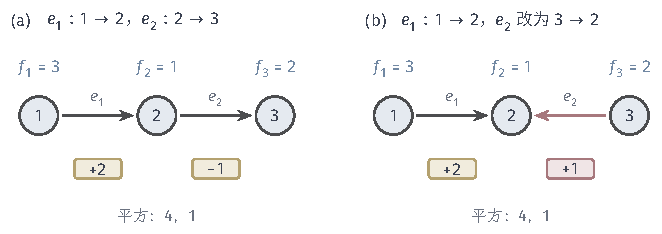
\includegraphics[width=112mm]{figures/01-basic-mathematics/04-graphs/tikz/c6-vertex-edge-functions/figure.pdf}
  \caption{三点路径上的顶点函数与边函数。蓝色数字是顶点值$\bm f=(3,1,2)^{\top}$，方框中是按参考方向计算的边差$(\bm B^{\top}\bm f)_e$（起点减终点）。(a)~$e_1:1\to2$、$e_2:2\to3$，边差为$(2,-1)$；(b)~只把$e_2$改记为$3\to2$（红色），它的边差变为$+1$。单条边差的符号随参考方向改变，平方$4$与$1$不变。}
  \label{fig:graph-spec-vertex-edge-functions}
\end{figure}

单条边差依赖参考方向。把$e_2$改记为$3\to2$，$\bm B$的第二列变号，该边的差从$f_2-f_3=-1$变成$f_3-f_2=1$，而$e_1$的差不受影响，见图~\ref{fig:graph-spec-vertex-edge-functions}。用矩阵表示，一次改记相当于右乘一个对角元为$\pm1$的符号矩阵$\bm R$（改记的边取$-1$），新关联矩阵为$\bm B\bm R$，新边差为$\bm R\bm B^{\top}\bm f$：每个分量至多变号，绝对值与平方都不变。由此得到构造无向图算子的一条要求：结果只能依赖边差的平方或其他不受符号影响的组合，否则它描述的是记账方式，而不是图本身。下一节的拉普拉斯满足这一要求。

% 第6章第2节：图拉普拉斯（邻域汇总、组合拉普拉斯、二次型与沿边变化能量）。

\section{图拉普拉斯}
\label{sec:graph-laplacian}

上一节得到了每条边上的差，但还没有把它们组织成作用于顶点函数的算子。本节沿两条路线构造同一个算子：一条在每个顶点读取邻居并与本点比较，另一条先取边差、再按边权缩放、最后汇总回顶点。两条路线的结果都是组合拉普拉斯，它的二次型累计各边差值的平方，用来衡量函数沿边变化的总量。

\subsection{邻域汇总}
\label{sec:graph-spec-neighborhood-aggregation}

最直接的图上运算是读取邻居。用权矩阵$\bm W$左乘顶点函数，
\[
 (\bm W\bm f)_i=\sum_{j=1}^nw_{i,j}f_j ,
\]
第$i$个输出把各邻居的值按边权加权求和；非邻居的$w_{i,j}=0$，不参与计算。与之相伴的量是顶点$i$的\term{加权度}（weighted degree）
\[
 d_i=\sum_{j=1}^nw_{i,j},\qquad \bm D=\operatorname{diag}(d_1,\ldots,d_n),
\]
它累计与$i$相连的全部边权。第~\ref{sec:graph-adjacency-paths}节的度数的是邻居个数，加权度数的是连接强度，只有每条边权都为$1$时二者才相等。本章后文所说的度一律指加权度。

$\bm W\bm f$是加权和，不是平均。在单位权三点路径上取$\bm f=(3,1,2)^{\top}$，得到$\bm W\bm f=(1,5,1)^{\top}$：中间顶点读到两个邻居之和$5$，比任何一个邻居的值都大。要得到邻居的平均，还须除以加权度，这是第~\ref{sec:graph-normalized-laplacian}节的工作。

\paragraph{同步读取与就地更新}
“作用一次”还有一个容易忽略的约定：所有顶点都从同一份旧向量读取，结果写入另一份新数组。若在原数组上就地按编号逐个更新，后更新的顶点会读到本轮已经改写的值。在上面的例子中按$1,2,3$的次序就地更新：先得$v_1=f_2=1$；更新顶点$2$时读到的是新值$v_1=1$而不是$3$，得$v_2=1+2=3$；再得$v_3=v_2=3$。结果是$(1,3,3)^{\top}$而不是$(1,5,1)^{\top}$。就地更新实现的是另一个与次序有关的映射，不再是$\bm W$。本章所说的算子作用都指同步读取旧值，只涉及一次线性映射，不涉及随时间演化的过程。

\subsection{组合拉普拉斯}
\label{sec:graph-spec-combinatorial-laplacian}

邻域汇总给出了邻居的加权和，衡量变化还需要把本点值与邻居值相比较。对每个邻居取差$f_i-f_j$，再按边权求和，得到
\[
 \sum_{j=1}^nw_{i,j}(f_i-f_j)=d_if_i-(\bm W\bm f)_i .
\]
右端对每个$i$成立，于是这一运算可以写成矩阵$\bm D-\bm W$。

\begin{definition}[组合拉普拉斯]
\label{def:graph-spec-combinatorial-laplacian}
设$\mathcal G=(V,E)$为有限无向图，边权对称非负、无自环，$\bm W$与$\bm D$分别为权矩阵与加权度矩阵。称
\begin{equation}
 \bm L=\bm D-\bm W
 \label{eq:graph-spec-laplacian}
\end{equation}
为$\mathcal G$的\term{组合图拉普拉斯}（combinatorial graph Laplacian），它逐点作用为$(\bm L\bm f)_i=\sum_jw_{i,j}(f_i-f_j)$。
\end{definition}

逐项看，$\bm L$的对角元是加权度$d_i$，非对角元是$-w_{i,j}$；每行之和为$d_i-\sum_jw_{i,j}=0$，所以$\bm L\bm1=\bm0$，常量函数被映成零。这与直觉一致：常量在每条边上都没有差。单位权三点路径的拉普拉斯为
\[
 \bm L=\begin{bmatrix}1&-1&0\\-1&2&-1\\0&-1&1\end{bmatrix},\qquad
 \bm L\begin{bmatrix}3\\1\\2\end{bmatrix}=\begin{bmatrix}2\\-3\\1\end{bmatrix}.
\]
中间顶点的输出$-3$是它与两个邻居之差的和$(1-3)+(1-2)$，负号表示它比邻居低。

\begin{figure}[!htb]
  \centering
  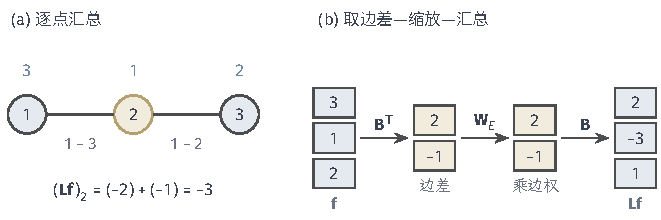
\includegraphics[width=112mm]{figures/01-basic-mathematics/04-graphs/tikz/c6-laplacian-two-routes/figure.pdf}
  \caption{同一个拉普拉斯的两条计算路线，单位权三点路径，$\bm f=(3,1,2)^{\top}$。(a)~在黄色顶点$2$处把本点值与每个邻居值相减再求和，得$(\bm L\bm f)_2=-3$；(b)~先用$\bm B^{\top}$取边差$(2,-1)$，再乘边权（此处均为$1$），最后用$\bm B$按净流出汇总回顶点，得到完整的$\bm L\bm f=(2,-3,1)^{\top}$。两条路线在每个顶点给出相同结果。}
  \label{fig:graph-spec-laplacian-two-routes}
\end{figure}

\paragraph{取边差、缩放、汇总}
第二条路线把上一节的边差接进来：先用$\bm B^{\top}$取边差，再用$\bm W_E$把第$e$条边的差乘以$w_e$，最后用$\bm B$按净流出汇总回顶点。三步合起来是矩阵$\bm B\bm W_E\bm B^{\top}$。为了核对它等于$\bm L$，记$\bm b_e$为$\bm B$的第$e$列，则
\[
 \bm B\bm W_E\bm B^{\top}=\sum_{e\in E}w_e\bm b_e\bm b_e^{\top}.
\]
若$e$连接$i$与$j$，则$\bm b_e=\pm(\bm e_i-\bm e_j)$，$\bm b_e\bm b_e^{\top}$在$(i,i)$、$(j,j)$处为$1$，在$(i,j)$、$(j,i)$处为$-1$，其余为零，而且与参考方向无关。逐边相加，每个对角位置累计出$d_i$，每个非对角位置得到$-w_{i,j}$，因此
\begin{equation}
 \bm L=\bm B\bm W_E\bm B^{\top}.
 \label{eq:graph-spec-laplacian-incidence}
\end{equation}
图~\ref{fig:graph-spec-laplacian-two-routes}在三点路径上并排执行了两条路线。

\paragraph{与参考方向无关}
上一节要求无向图算子不依赖参考方向，式~\eqref{eq:graph-spec-laplacian-incidence}可以整体核对这一点。改记部分边的方向后，关联矩阵变为$\bm B\bm R$，其中$\bm R$是对角元为$\pm1$的符号矩阵。由于对角矩阵相乘可以交换、$\bm R^2=\bm I$，有$\bm R\bm W_E\bm R=\bm W_E$，于是
\[
 (\bm B\bm R)\bm W_E(\bm B\bm R)^{\top}=\bm B\bm R\bm W_E\bm R\bm B^{\top}=\bm B\bm W_E\bm B^{\top}.
\]
边差变号了两次，一次在取差时，一次在汇总时，两次抵消。这一抵消依赖于参考方向只是记账约定；对真正的有向图，弧的方向是数据本身，不能用同样的理由消去，有向图的拉普拉斯一般不对称，不在本章范围内。

\subsection{二次型与沿边变化能量}
\label{sec:graph-spec-dirichlet-energy}

有了算子，再看它的二次型能说明什么。把式~\eqref{eq:graph-spec-laplacian-incidence}代入$\bm f^{\top}\bm L\bm f$，中间恰好是边差的加权平方和：
\begin{equation}
 \begin{aligned}
 \bm f^{\top}\bm L\bm f
 &=(\bm B^{\top}\bm f)^{\top}\bm W_E(\bm B^{\top}\bm f)
 =\sum_{\{i,j\}\in E}w_{i,j}(f_i-f_j)^2\\
 &=\frac12\sum_{i=1}^n\sum_{j=1}^nw_{i,j}(f_i-f_j)^2 .
 \end{aligned}
 \label{eq:graph-spec-dirichlet-energy}
\end{equation}
中间的和对无向边求和，每条边计一次；最右端对有序点对$(i,j)$求和，每条边作为$(i,j)$与$(j,i)$各出现一次，所以要乘$\frac12$。这个量称为沿边变化能量，也称\term{Dirichlet能量}（Dirichlet energy）。它的大小取决于两样东西：相邻值差多少，以及图要求这一对顶点被比较得多强。

\begin{figure}[!htb]
  \centering
  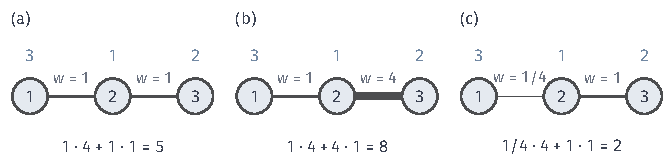
\includegraphics[width=112mm]{figures/01-basic-mathematics/04-graphs/tikz/c6-energy-edge-weights/figure.pdf}
  \caption{同一顶点函数$\bm f=(3,1,2)^{\top}$在三组边权下的沿边变化能量，线宽示意边权大小。两条边的差的平方始终为$4$与$1$，能量是它们的加权和：(a)~权$(1,1)$时为$5$；(b)~加重边$\{2,3\}$后为$8$；(c)~减轻边$\{1,2\}$后为$2$。}
  \label{fig:graph-spec-energy-edge-weights}
\end{figure}

图~\ref{fig:graph-spec-energy-edge-weights}固定$\bm f=(3,1,2)^{\top}$，只改变边权。两条边的差的平方始终是$4$和$1$。单位权时能量为$4+1=5$；把$\{2,3\}$的权加到$4$，较小的差被放大四倍，能量变为$4+4=8$；把$\{1,2\}$的权减到$\frac14$，较大的差几乎不再计入，能量降到$1+1=2$。所以说一个函数“平滑”，总是相对于给定的边权而言的。

\paragraph{半正定与零能量}
式~\eqref{eq:graph-spec-dirichlet-energy}的每一项都是非负权乘平方，所以对任意$\bm f$都有$\bm f^{\top}\bm L\bm f\geq0$。$\bm L$又是对称矩阵，因此它对称半正定（第~\ref{sec:ls-gram-psd}节）。这一结论用到了权非负：若允许负权，对应的项可以为负，半正定性一般不再成立。

能量何时为零？各项非负，总和为零当且仅当每一项为零，即对每条正权边都有$f_i=f_j$；零权边的项本来就是零，不对两端施加任何限制。这是逐边的条件。相等关系怎样沿正权路径传递，零能量的函数究竟有哪些，要用到连通分量，留到第~\ref{sec:graph-spectrum-connectivity}节统一回答。

% 第6章第3节：归一化拉普拉斯（度加权内积、对称归一化拉普拉斯、随机游走拉普拉斯、两种归一化的联系）。

\section{归一化拉普拉斯}
\label{sec:graph-normalized-laplacian}

组合拉普拉斯平等对待每个顶点上的数值。当各顶点的连接总量相差很大时，这种平等会带来偏差：改变连接多的顶点上的值，会同时牵动许多条边。本节先用度给长度加权，再经坐标缩放得到对称归一化拉普拉斯，然后从邻域平均得到随机游走拉普拉斯，最后说明二者的关系。

下面的公式要对加权度取倒数或倒数平方根，只对正度顶点有意义。记$V_+=\{i\in V:d_i>0\}$。度为零的顶点没有任何正权邻边，它在正权支撑图中是孤立点，下文称为支撑孤点；结构上它可能仍连着零权边。每个公式先在正度顶点上建立，再单独约定支撑孤点的处理。

\subsection{度加权内积}
\label{sec:graph-spec-degree-inner-product}

先看连接多少怎样影响能量。图~\ref{fig:graph-spec-degree-weighted-length}是单位权星图，中心连着三片叶，中心的度为$3$，叶的度为$1$。只在中心放一个单位值时，三条边都出现差$1$，能量为$3$；只在一片叶上放同样的单位值，只有一条边有差，能量为$1$。两个函数的欧氏长度都是$1$，能量却相差三倍。原因不在数值本身，而在中心连接更多：同样大小的改动，放在高度顶点上要被更多条边计入。

\begin{figure}[!htb]
  \centering
  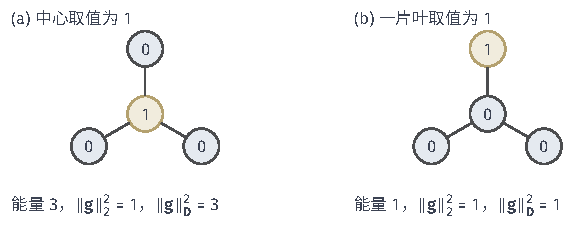
\includegraphics[width=97mm]{figures/01-basic-mathematics/04-graphs/tikz/c6-degree-weighted-length/figure.pdf}
  \caption{单位权星图上的两个单位脉冲，黄色顶点取值$1$，其余为$0$。(a)~中心的度为$3$，能量为$3$；(b)~叶的度为$1$，能量为$1$。两者的欧氏长度平方都是$1$，按度加权的长度平方分别为$3$和$1$，与能量成相同比例。}
  \label{fig:graph-spec-degree-weighted-length}
\end{figure}

如果在衡量函数大小时也把连接量计入，用$\sum_id_ig_i^2$代替$\sum_ig_i^2$，两个脉冲的长度平方就分别是$3$和$1$，能量与长度之比都等于$1$。这提示了一种新的内积：对定义在$V_+$上的函数，令
\begin{equation}
 \langle\bm g,\bm h\rangle_{\bm D}=\bm g^{\top}\bm D\bm h=\sum_{i\in V_+}d_ig_ih_i .
 \label{eq:graph-spec-degree-inner-product}
\end{equation}
在$V_+$上$\bm D$是正对角矩阵，因而对称正定，这正是第~\ref{sec:ls-weighted-inner-products}节的加权内积，称为\term{度加权内积}（degree-weighted inner product）。它与欧氏内积的区别只在于每个顶点的贡献乘以了该点的度。

加权内积可以换回普通内积，办法是缩放坐标。令$\bm f=\bm D^{1/2}\bm g$，即$f_i=\sqrt{d_i}\,g_i$，则
\[
 \lVert\bm f\rVert_2^2=\sum_id_ig_i^2=\bm g^{\top}\bm D\bm g=\lVert\bm g\rVert_{\bm D}^2 .
\]
在新坐标$\bm f$中，度加权长度就是欧氏长度，第三部分关于欧氏内积和对称矩阵的结论可以直接使用。含支撑孤点时，$\bm D$在整个$\mathbb R^n$上是奇异的：取$\bm g$为孤点$v$处的坐标向量$\bm e_v$，有$\bm g^{\top}\bm D\bm g=d_v=0$而$\bm g\neq\bm0$，正定性不成立。所以式~\eqref{eq:graph-spec-degree-inner-product}只在$V_+$上是内积，不能直接称为全空间的内积。

\subsection{对称归一化拉普拉斯}
\label{sec:graph-spec-symmetric-normalized}

先在全体顶点度为正的情形下推导。函数$\bm g$的能量是$\bm g^{\top}\bm L\bm g$，它的度加权长度平方是$\bm g^{\top}\bm D\bm g$。把坐标代换$\bm g=\bm D^{-1/2}\bm f$代入两者，得到
\[
 \frac{\bm g^{\top}\bm L\bm g}{\bm g^{\top}\bm D\bm g}
 =\frac{\bm f^{\top}\bm D^{-1/2}\bm L\bm D^{-1/2}\bm f}{\bm f^{\top}\bm f}.
\]
左端按度衡量的“每单位长度的能量”，在新坐标中变成了一个对称矩阵的普通Rayleigh商（定义~\ref{def:matrix-analysis-rayleigh-quotient}）。这个对称矩阵就是要找的算子。

\begin{definition}[对称归一化拉普拉斯]
\label{def:graph-spec-symmetric-normalized-laplacian}
设全体顶点的加权度为正，称
\begin{equation}
 \bm L_{\mathrm{sym}}=\bm D^{-1/2}\bm L\bm D^{-1/2}=\bm I-\bm D^{-1/2}\bm W\bm D^{-1/2}
 \label{eq:graph-spec-symmetric-normalized-laplacian}
\end{equation}
为\term{对称归一化拉普拉斯}（symmetric normalized Laplacian）。它的对角元为$1$，$(i,j)$位置的非对角元为$-w_{i,j}/\sqrt{d_id_j}$。
\end{definition}

逐边展开它的二次型，可以看出它比较的是什么。$\bm f^{\top}\bm L_{\mathrm{sym}}\bm f$就是$\bm g=\bm D^{-1/2}\bm f$的能量$\bm g^{\top}\bm L\bm g$，把$g_i=f_i/\sqrt{d_i}$代入式~\eqref{eq:graph-spec-dirichlet-energy}，得到
\begin{equation}
 \bm f^{\top}\bm L_{\mathrm{sym}}\bm f=\sum_{\{i,j\}\in E_+}w_{i,j}\left(\frac{f_i}{\sqrt{d_i}}-\frac{f_j}{\sqrt{d_j}}\right)^2\geq0 .
 \label{eq:graph-spec-normalized-energy}
\end{equation}
组合拉普拉斯比较的是相邻顶点的原值，$\bm L_{\mathrm{sym}}$比较的是先除以$\sqrt{d_i}$后的值。求和只经过正权边，而正权边的两个端点度都为正，分母不会出现零。

\paragraph{支撑孤点的约定}
有支撑孤点时，式~\eqref{eq:graph-spec-symmetric-normalized-laplacian}中的$\bm D^{-1/2}$无法按原样定义。约定$\bm D^{-1/2}$是对角矩阵，正度顶点处取$d_i^{-1/2}$，支撑孤点处取$0$，再用$\bm L_{\mathrm{sym}}=\bm D^{-1/2}\bm L\bm D^{-1/2}$定义。支撑孤点$v$在$\bm L$中的行和列本来全为零，在$\bm L_{\mathrm{sym}}$中也全为零，于是对角元$(\bm L_{\mathrm{sym}})_{v,v}=0$。在这一约定下，第二种写法$\bm I-\bm D^{-1/2}\bm W\bm D^{-1/2}$会在孤点处给出$1$，二者不再相同，所以有支撑孤点时只用第一种写法。

以单位权路径$1-2-3$外加孤立顶点$4$为例，度为$(1,2,1,0)$，按约定$\bm D^{-1/2}=\operatorname{diag}(1,\tfrac1{\sqrt2},1,0)$，于是
\[
 \bm L_{\mathrm{sym}}=\begin{bmatrix}1&-\tfrac1{\sqrt2}&0&0\\-\tfrac1{\sqrt2}&1&-\tfrac1{\sqrt2}&0\\0&-\tfrac1{\sqrt2}&1&0\\0&0&0&0\end{bmatrix}.
\]
它的第四行、第四列全为零。二次型~\eqref{eq:graph-spec-normalized-energy}只经过边$\{1,2\}$、$\{2,3\}$，与这个矩阵一致：$f_4$不出现在任何一项中。孤点给$\bm L_{\mathrm{sym}}$带来一个零特征值，它的谱留到第~\ref{sec:graph-spectrum-connectivity}节统一讨论。

\subsection{随机游走拉普拉斯}
\label{sec:graph-spec-random-walk-laplacian}

第~\ref{sec:graph-spec-neighborhood-aggregation}小节指出$\bm W\bm f$是加权和而不是平均。在正度顶点上把第$i$行除以$d_i$，就得到平均：
\[
 \bm P_{\mathrm{rw}}=\bm D^{-1}\bm W,\qquad
 (\bm P_{\mathrm{rw}}\bm f)_i=\sum_j\frac{w_{i,j}}{d_i}f_j .
\]
这里的下标与重编号用的置换矩阵$\bm P$相区别。$\bm P_{\mathrm{rw}}$每行的权非负且和为$1$，所以$(\bm P_{\mathrm{rw}}\bm f)_i$是邻居值的加权平均，介于邻居值的最小值与最大值之间。支撑孤点没有邻居可平均，约定$(\bm P_{\mathrm{rw}})_{v,v}=1$、该行其余元素为$0$，使孤点保持原值。在单位权三点路径上，$\bm P_{\mathrm{rw}}(3,1,2)^{\top}=(1,\tfrac52,1)^{\top}$：中间顶点得到两个邻居的平均$\tfrac52$，不再是和$5$。

本点值减去邻居平均，就得到第三个算子
\begin{equation}
 \bm L_{\mathrm{rw}}=\bm I-\bm P_{\mathrm{rw}} ,
 \label{eq:graph-spec-random-walk-laplacian}
\end{equation}
称为\term{随机游走拉普拉斯}（random-walk Laplacian）。在正度顶点的行上，$\bm L_{\mathrm{rw}}=\bm D^{-1}\bm L$，即$(\bm L_{\mathrm{rw}}\bm f)_i=(\bm L\bm f)_i/d_i$；支撑孤点的行全为零。上例中$\bm L_{\mathrm{rw}}(3,1,2)^{\top}=(2,-\tfrac32,1)^{\top}$，中间顶点的输出是$1-\tfrac52$。

名称中的“随机游走”来自对$w_{i,j}/d_i$的一种解释：把它看成从$i$出发下一步走到$j$的概率。完整的随机游走还需要随机序列和转移规则，它的稳态与收敛属于后续概率部分。本节只使用有限个非负权的加权平均，不涉及任何随机性或收敛结论。

\subsection{两种归一化的联系}
\label{sec:graph-spec-normalization-relations}

$\bm L_{\mathrm{sym}}$由坐标缩放得到，$\bm L_{\mathrm{rw}}$由邻域平均得到，两者其实是同一个作用的两种写法。在正度顶点上，
\[
 \bm D^{-1/2}\bm L_{\mathrm{sym}}\bm D^{1/2}=\bm D^{-1/2}\bm D^{-1/2}\bm L\bm D^{-1/2}\bm D^{1/2}=\bm D^{-1}\bm L=\bm L_{\mathrm{rw}} .
\]
所以二者相似（第~\ref{sec:ls-similarity}节），特征值相同，特征向量要经坐标转换：若$\bm L_{\mathrm{sym}}\bm x=\lambda\bm x$，则$\bm L_{\mathrm{rw}}(\bm D^{-1/2}\bm x)=\lambda\bm D^{-1/2}\bm x$。读法是：$\bm L_{\mathrm{rw}}$作用于原坐标$\bm g$，等于先换到$\bm f=\bm D^{1/2}\bm g$，用$\bm L_{\mathrm{sym}}$作用，再换回原坐标。

$\bm L_{\mathrm{rw}}$一般不对称。单位权三点路径上，它的$(1,2)$元是$-1$，$(2,1)$元是$-\tfrac12$。但它在度加权内积下自伴（第~\ref{sec:ls-adjoints}节）：由$\bm D\bm L_{\mathrm{rw}}=\bm L=\bm L^{\top}$，
\[
 \langle\bm L_{\mathrm{rw}}\bm g,\bm h\rangle_{\bm D}=\bm g^{\top}\bm L_{\mathrm{rw}}^{\top}\bm D\bm h=\bm g^{\top}\bm L\bm h=\langle\bm g,\bm L_{\mathrm{rw}}\bm h\rangle_{\bm D} .
\]
有支撑孤点时，这些关系都限制在正度顶点上成立。

\begin{figure}[!htb]
  \centering
  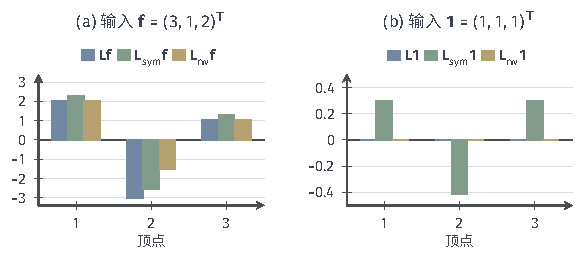
\includegraphics[width=98mm]{figures/01-basic-mathematics/04-graphs/tikz/c6-three-laplacians/figure.pdf}
  \caption{单位权三点路径（度为$1,2,1$）上三种拉普拉斯作用于同一向量。(a)~输入$(3,1,2)^{\top}$：$\bm L_{\mathrm{rw}}$把$\bm L$的输出逐点除以度，中间顶点从$-3$变为$-\tfrac32$；$\bm L_{\mathrm{sym}}$的输出约为$(2.29,-2.54,1.29)$。(b)~输入常量$\bm1$：$\bm L$与$\bm L_{\mathrm{rw}}$都给出零，$\bm L_{\mathrm{sym}}$不给出零。}
  \label{fig:graph-spec-three-laplacians}
\end{figure}

用一个度不相等的例子对照三个算子。单位权三点路径的度为$(1,2,1)$，图~\ref{fig:graph-spec-three-laplacians}(a)把它们作用于$\bm f=(3,1,2)^{\top}$：
\[
 \bm L\bm f=\begin{bmatrix}2\\-3\\1\end{bmatrix},\quad
 \bm L_{\mathrm{rw}}\bm f=\begin{bmatrix}2\\-\tfrac32\\1\end{bmatrix},\quad
 \bm L_{\mathrm{sym}}\bm f=\begin{bmatrix}3-\tfrac1{\sqrt2}\\1-\tfrac5{\sqrt2}\\2-\tfrac1{\sqrt2}\end{bmatrix}\approx\begin{bmatrix}2.29\\-2.54\\1.29\end{bmatrix}.
\]
$\bm L_{\mathrm{rw}}$只是把$\bm L$的输出逐点除以度，度为$1$的端点不变；$\bm L_{\mathrm{sym}}$则先把输入缩放成$\bm D^{-1/2}\bm f=(3,\tfrac1{\sqrt2},2)^{\top}$，再作用、再缩放，每个分量都变了。图~(b)换成常量输入$\bm1$：$\bm L\bm1=\bm L_{\mathrm{rw}}\bm1=\bm0$，而$\bm L_{\mathrm{sym}}\bm1=(1-\tfrac1{\sqrt2},1-\sqrt2,1-\tfrac1{\sqrt2})^{\top}\neq\bm0$。$\bm L_{\mathrm{sym}}$消去的是度缩放后的常量$\bm D^{1/2}\bm1=(1,\sqrt2,1)^{\top}$，因为$\bm L_{\mathrm{sym}}\bm D^{1/2}\bm1=\bm D^{-1/2}\bm L\bm1=\bm0$。

这个例子区分了三件不同的事。从$\bm L$到$\bm L_{\mathrm{rw}}$是改变算子：输出被逐点除以度，零向量不变，但输出的尺度变了。从$\bm L_{\mathrm{rw}}$到$\bm L_{\mathrm{sym}}$是改变坐标：同一个作用在$\bm g$坐标与$\bm f=\bm D^{1/2}\bm g$坐标中分别写成这两个矩阵。把欧氏内积换成度加权内积则是改变内积：$\bm L_{\mathrm{rw}}$在欧氏内积下不对称，在度加权内积下自伴。后面选取谱基、作谱划分时，都要先说明用的是哪个算子、哪种坐标。

% 第6章第4节：图谱与连通性（特征向量与变化尺度、零空间与连通分量、归一化谱界）。

\section{图谱与连通性}
\label{sec:graph-spectrum-connectivity}

前两节建立的$\bm L$与$\bm L_{\mathrm{sym}}$都是实对称矩阵，可以直接使用第三部分的谱定理。本节回答三个问题：特征向量表示怎样的变化模式，零特征值反映了图的什么结构，归一化后的特征值落在什么范围。所选图算子的特征值合起来称为\term{图谱}（graph spectrum）。它由算子和边权决定，不由顶点编号决定，也不是事先给定的物理频率。

\subsection{特征向量与变化尺度}
\label{sec:graph-spec-eigenvectors-scales}

由谱定理（定理~\ref{thm:ls-real-symmetric-spectral}），存在正交矩阵$\bm U=[\bm u_1,\ldots,\bm u_n]$与实对角矩阵$\bm\Lambda$，使
\begin{equation}
 \bm L=\bm U\bm\Lambda\bm U^{\top},\qquad
 \bm\Lambda=\operatorname{diag}(\lambda_1,\ldots,\lambda_n),\qquad
 \lambda_1\leq\lambda_2\leq\cdots\leq\lambda_n .
 \label{eq:graph-spec-laplacian-eigendecomposition}
\end{equation}
按本章约定，特征值从小到大编号。$\bm L$半正定，所以全部$\lambda_k\geq0$；又$\bm L\bm1=\bm0$，所以$\lambda_1=0$。

特征值有一个直接的含义。对单位特征向量$\bm u_k$，
\[
 \bm u_k^{\top}\bm L\bm u_k=\lambda_k\bm u_k^{\top}\bm u_k=\lambda_k ,
\]
即$\lambda_k$就是$\bm u_k$的沿边变化能量。由于长度已经固定为$1$，小特征值对应沿边起伏小的方向，大特征值对应相邻顶点取值差异大的方向。因此常把$\lambda_k$称为\term{图频率}（graph frequency）：把特征值看作频率，特征向量看作该频率的振荡模式，低频平缓、高频剧烈。

\begin{figure}[!htb]
  \centering
  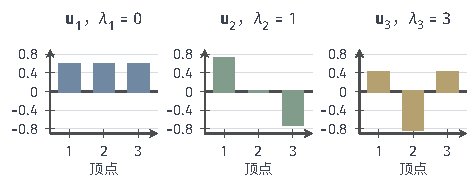
\includegraphics[width=80mm]{figures/01-basic-mathematics/04-graphs/tikz/c6-path-modes/figure.pdf}
  \caption{单位权三点路径的三个标准正交特征向量，条高为各顶点上的取值。$\bm u_1$为常量，能量$0$；$\bm u_2$两端反号、中间为零，变号一次，能量$1$；$\bm u_3$中间与两端反号，变号两次，能量$3$。}
  \label{fig:graph-spec-path-modes}
\end{figure}

单位权三点路径的拉普拉斯可以逐个核对。取
\[
 \bm u_1=\tfrac1{\sqrt3}(1,1,1)^{\top},\qquad
 \bm u_2=\tfrac1{\sqrt2}(1,0,-1)^{\top},\qquad
 \bm u_3=\tfrac1{\sqrt6}(1,-2,1)^{\top}.
\]
直接相乘得$\bm L(1,0,-1)^{\top}=(1,0,-1)^{\top}$、$\bm L(1,-2,1)^{\top}=(3,-6,3)^{\top}$，所以对应特征值为$0,1,3$。用能量逐边核对：$\bm u_2$在两条边上的差都是$\tfrac1{\sqrt2}$，能量$\tfrac12+\tfrac12=1$；$\bm u_3$在两条边上的差都是$\tfrac3{\sqrt6}$，能量$\tfrac96+\tfrac96=3$。图~\ref{fig:graph-spec-path-modes}显示，从常量到左右反向、再到中间与两端反向，变号次数增加，能量随之增大。

图频率依赖边权。把边$\{2,3\}$的权从$1$改为$4$，拉普拉斯变为
\[
 \begin{bmatrix}1&-1&0\\-1&5&-4\\0&-4&4\end{bmatrix},
\]
除零之外的两个特征值满足$\lambda^2-10\lambda+12=0$，即$5\pm\sqrt{13}\approx1.39,\,8.61$。连接关系和顶点次序都没变，谱却变了。所以不能把图频率看成只由无权连接或数组次序决定的固定量。

\paragraph{重编号下的谱}
第~\ref{sec:graph-isomorphism}节用置换矩阵$\bm P$表示顶点重编号，邻接矩阵变为$\bm P\bm A\bm P^{\top}$。度矩阵与权矩阵同步重排，所以拉普拉斯变为$\bm L'=\bm P\bm L\bm P^{\top}$。若$\bm L\bm u=\lambda\bm u$，由$\bm P^{\top}\bm P=\bm I$，
\[
 \bm L'(\bm P\bm u)=\bm P\bm L\bm P^{\top}\bm P\bm u=\bm P\bm L\bm u=\lambda\,\bm P\bm u .
\]
特征值不变，特征向量的分量随顶点一起重排。这区分了三个层次：记录顺序是任意选择的；特征向量在某个记录顺序下的坐标随顺序改变；图谱本身则不依赖记录顺序，是同构图共有的量。

\subsection{零空间与连通分量}
\label{sec:graph-spec-null-space-components}

第~\ref{sec:graph-spec-dirichlet-energy}小节得到了逐边条件：能量为零当且仅当每条正权边两端相等。把这个条件沿路径传递，就能确定全部零特征向量。下面的$\bm1_C$表示顶点集$C$的指示向量，在$C$上取$1$、其余为$0$；连通分量的概念见第~\ref{sec:graph-connectivity-separation}节。

\begin{theorem}[零空间与正权支撑分量]
\label{thm:graph-spec-null-space}
设$\mathcal G$为有限无向图，边权非负对称，正权支撑图$(V,E_+)$的连通分量为$C_1,\ldots,C_c$，则
\[
 \ker\bm L=\operatorname{span}\{\bm1_{C_1},\ldots,\bm1_{C_c}\},
\]
且$\bm L$的零特征值的重数等于$c$。
\end{theorem}

\begin{proof}
第一步，零空间由能量刻画。若$\bm L\bm f=\bm0$，则$\bm f^{\top}\bm L\bm f=\bm f^{\top}\bm0=0$。反过来，把$\bm f=\sum_kc_k\bm u_k$代入，$\bm f^{\top}\bm L\bm f=\sum_k\lambda_kc_k^2$，各项非负，和为零迫使$\lambda_k>0$时$c_k=0$，于是$\bm L\bm f=\sum_k\lambda_kc_k\bm u_k=\bm0$。所以$\bm L\bm f=\bm0$当且仅当$\bm f^{\top}\bm L\bm f=0$，又当且仅当每条正权边两端相等。

第二步，相等关系沿路径传递。若$i$与$j$在同一分量$C$中，则存在一条只经过正权边的路径$i=v_0,v_1,\ldots,v_\ell=j$，逐边得$f_{v_0}=f_{v_1}=\cdots=f_{v_\ell}$。所以零能量的函数在每个分量上取常数。反之，正权边的两个端点总在同一分量中，在各分量上分别取常数的函数，在每条正权边上的差都为零。于是$\ker\bm L$恰为“在每个分量上取常数”的函数全体，每个这样的函数都可写成$\sum_ta_t\bm1_{C_t}$。

第三步，数维数。各分量互不相交，指示向量的支撑互不重叠，两两正交，因而线性无关，$\dim\ker\bm L=c$。在谱分解~\eqref{eq:graph-spec-laplacian-eigendecomposition}中，$\ker\bm L$由$\lambda_k=0$的那些$\bm u_k$张成，所以零特征值恰好出现$c$次。
\end{proof}

这一结论特别给出：$\lambda_2>0$当且仅当正权支撑图连通。图~\ref{fig:graph-spec-component-null-modes}中的图有三个正权支撑分量：路径$\{1,2,3\}$、边$\{4,5\}$和孤点$6$，所以零特征值的重数为$3$（直接计算可得$\bm L$的谱为$0,0,0,1,2,3$）。连接$3$与$4$的零权边结构上存在，但它的能量项恒为零，不迫使两端相等，所以不能把两个分量合并：$\bm1_{C_1}$与$\bm1_{C_2}$可以分别取不同的常数。

\begin{figure}[!htb]
  \centering
  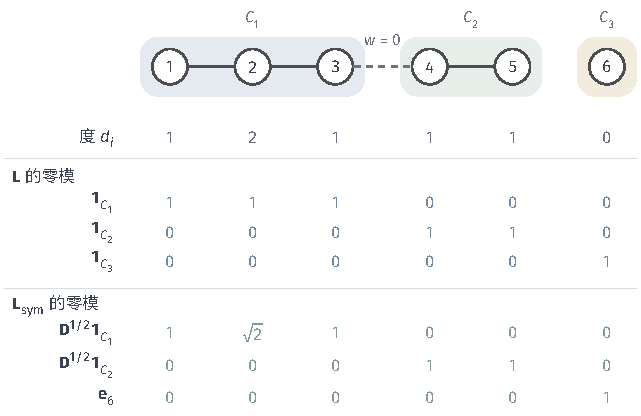
\includegraphics[width=108mm]{figures/01-basic-mathematics/04-graphs/tikz/c6-component-null-modes/figure.pdf}
  \caption{正权支撑分量与零特征向量。实线为单位权边，虚线$\{3,4\}$为零权结构边，顶点$6$为支撑孤点；三块底色标出分量$C_1,C_2,C_3$。上半部分为$\bm L$零空间的一组基，即各分量的指示向量；下半部分为$\bm L_{\mathrm{sym}}$零空间的一组基：正度分量上是度缩放的指示向量$\bm D^{1/2}\bm1_C$，孤点处是坐标方向$\bm e_6$。两组基的个数相同，向量不同。}
  \label{fig:graph-spec-component-null-modes}
\end{figure}

\paragraph{归一化算子的零空间}
同样的论证可以搬到$\bm L_{\mathrm{sym}}$。在正度顶点上，由式~\eqref{eq:graph-spec-normalized-energy}，能量为零当且仅当每条正权边上$f_i/\sqrt{d_i}=f_j/\sqrt{d_j}$，即$\bm D^{-1/2}\bm f$在每个分量上取常数。所以每个含正权边的分量$C$贡献零特征向量$\bm D^{1/2}\bm1_C$。支撑孤点$v$的行与列全为零，坐标方向$\bm e_v$也是零特征向量。合起来，$\bm L_{\mathrm{sym}}$的零特征值重数仍等于正权支撑分量数（孤点自成一个分量），但基向量换成了度缩放的版本。图~\ref{fig:graph-spec-component-null-modes}的下半部分列出了它们，例如$\bm D^{1/2}\bm1_{C_1}=(1,\sqrt2,1,0,0,0)^{\top}$。

普通常量与度缩放常量不能互换。图~\ref{fig:graph-spec-three-laplacians}(b)已经显示$\bm L_{\mathrm{sym}}\bm1\neq\bm0$；只有在一个分量内各点度相同时，二者才成比例。至于$\bm L_{\mathrm{rw}}$，它在正度行上等于$\bm D^{-1}\bm L$，在孤点行上为零，所以$\bm L_{\mathrm{rw}}\bm g=\bm0$当且仅当$\bm L\bm g=\bm0$，零空间仍由普通的分量指示向量张成。

\subsection{归一化谱界}
\label{sec:graph-spec-normalized-bound}

组合拉普拉斯的特征值随边权整体放缩：所有边权乘以$c>0$，$\bm L$乘以$c$，谱也乘以$c$。$\bm L_{\mathrm{sym}}$则不受这种放缩影响，因为$\bm D^{-1/2}$同时乘以$c^{-1/2}$，两侧抵消。下面证明它的特征值总在一个固定区间内。

\begin{theorem}[归一化谱界]
\label{thm:graph-spec-normalized-bound}
对有限无向非负权图，按本节约定定义的$\bm L_{\mathrm{sym}}$满足$0\leq\bm f^{\top}\bm L_{\mathrm{sym}}\bm f\leq2\lVert\bm f\rVert_2^2$，因此它的全部特征值落在$[0,2]$中。
\end{theorem}

\begin{proof}
下界即式~\eqref{eq:graph-spec-normalized-energy}的非负性。对上界，对任意实数$a,b$有$(a-b)^2\leq2(a^2+b^2)$，因为两边之差为$(a+b)^2\geq0$。令$a_i=f_i/\sqrt{d_i}$（$i\in V_+$），逐边使用这一不等式：
\[
 \begin{aligned}
 \sum_{\{i,j\}\in E_+}w_{i,j}(a_i-a_j)^2
 &\leq2\sum_{\{i,j\}\in E_+}w_{i,j}\bigl(a_i^2+a_j^2\bigr)
 =2\sum_{i\in V_+}a_i^2\sum_jw_{i,j}\\
 &=2\sum_{i\in V_+}\frac{f_i^2}{d_i}\,d_i\leq2\lVert\bm f\rVert_2^2 .
 \end{aligned}
\]
中间的等号把每条边上的两项分别归到两个端点，每个顶点$i$收集到的权之和恰为$d_i$；最后一步只是丢掉了支撑孤点上的非负项$f_v^2$。设$\bm x_k$是$\bm L_{\mathrm{sym}}$的单位特征向量，特征值为$\mu_k$，取$\bm f=\bm x_k$即得$0\leq\mu_k=\bm x_k^{\top}\bm L_{\mathrm{sym}}\bm x_k\leq2$；也可以由Rayleigh--Ritz定理（定理~\ref{thm:matrix-analysis-rayleigh-ritz}）读出。
\end{proof}

上界可以取到。单位权三点路径的$\bm L_{\mathrm{sym}}$特征值为$0,1,2$，取到$2$的特征向量是$(1,-\sqrt2,1)^{\top}$，换回原坐标$\bm D^{-1/2}\bm f=(1,-1,1)^{\top}$，相邻顶点正负交替，每条边都达到证明中不等式的等号$a_i=-a_j$。组合拉普拉斯没有同样的统一上界：这条路径的$\bm L$已有特征值$3>2$。同样的论证只给出$\bm f^{\top}\bm L\bm f\leq2\sum_id_if_i^2\leq2d_{\max}\lVert\bm f\rVert_2^2$，上界随最大度和边权的尺度变化。

谱界告诉我们特征值可能出现在哪个区间。第~\ref{sec:graph-filtering}节设计滤波响应、用多项式逼近响应时，只需在这个区间上考虑。谱界本身不是任何迭代算法的收敛保证，那需要另行分析。

% 第6章第5节：图傅里叶变换（谱坐标与重构、环图上的傅里叶基）。

\section{图傅里叶变换}
\label{sec:graph-fourier-transform}
\label{sec:signal-analysis-graph-state-kernels}

上一节的特征向量按变化尺度排成一组标准正交基。本节把顶点函数展开在这组基上：先建立投影系数、重构公式和两种能量的分解，再在规则的环图上说明熟悉的复指数为什么恰好是特征向量。所用的只是有限维正交分解与复数运算，离散傅里叶变换和快速算法留给后续信号部分。

\subsection{谱坐标与重构}
\label{sec:graph-spec-spectral-coordinates}

给定$\bm L$的一组标准正交特征向量$\bm u_1,\ldots,\bm u_n$，按特征值从小到大排成正交矩阵$\bm U$。任意顶点函数都可以在这组基下写出坐标，坐标就是它与各基向量的内积（第~\ref{sec:ls-orthonormal-bases}节）。

\begin{definition}[图傅里叶变换]
\label{def:graph-spec-graph-fourier-transform}
设$\bm L=\bm U\bm\Lambda\bm U^{\top}$为式~\eqref{eq:graph-spec-laplacian-eigendecomposition}的谱分解。顶点函数$\bm f$的\term{图傅里叶变换}（graph Fourier transform）及其逆变换为
\begin{equation}
 \widehat{\bm f}=\bm U^{\top}\bm f,\qquad \bm f=\bm U\widehat{\bm f}=\sum_{k=1}^n\widehat f_k\bm u_k ,
 \label{eq:graph-spec-graph-fourier-transform}
\end{equation}
其中$\widehat f_k=\bm u_k^{\top}\bm f$称为$\bm f$的第$k$个\term{谱坐标}（spectral coordinate）。
\end{definition}

正变换逐个读出$\bm f$在各模态方向上的分量，逆变换再把这些分量乘回对应的基向量相加。因为$\bm U^{\top}\bm U=\bm U\bm U^{\top}=\bm I$，两步互为逆运算，完整换坐标不丢失任何信息。

\begin{figure}[!htb]
  \centering
  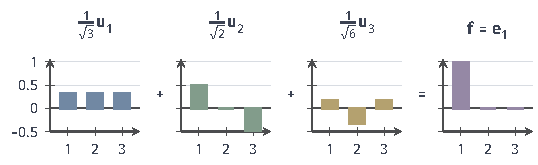
\includegraphics[width=91mm]{figures/01-basic-mathematics/04-graphs/tikz/c6-spectral-projection/figure.pdf}
  \caption{三点路径上单位脉冲的谱展开。前三幅是各模态乘以对应谱坐标后的贡献$\widehat f_k\bm u_k$，分别为$(\tfrac13,\tfrac13,\tfrac13)$、$(\tfrac12,0,-\tfrac12)$与$(\tfrac16,-\tfrac13,\tfrac16)$；逐点相加恰好恢复第四幅的$\bm e_1=(1,0,0)^{\top}$。}
  \label{fig:graph-spec-spectral-projection}
\end{figure}

在单位权三点路径上用第~\ref{sec:graph-spec-eigenvectors-scales}小节的三个模态展开单位脉冲$\bm f=\bm e_1$。三个谱坐标是$\bm u_k$的第一个分量：
\[
 \widehat{\bm f}=\Bigl(\tfrac1{\sqrt3},\tfrac1{\sqrt2},\tfrac1{\sqrt6}\Bigr)^{\top}.
\]
重构时，三个贡献分别是$\tfrac1{\sqrt3}\bm u_1=\tfrac13(1,1,1)^{\top}$、$\tfrac1{\sqrt2}\bm u_2=\tfrac12(1,0,-1)^{\top}$、$\tfrac1{\sqrt6}\bm u_3=\tfrac16(1,-2,1)^{\top}$。第一个分量相加为$\tfrac13+\tfrac12+\tfrac16=1$，第二个为$\tfrac13+0-\tfrac13=0$，第三个为$\tfrac13-\tfrac12+\tfrac16=0$，恰好回到$\bm e_1$，见图~\ref{fig:graph-spec-spectral-projection}。一个集中在一点的函数，需要全部三个模态共同表示。

\paragraph{两种能量的分解}
谱坐标把两种不同的“大小”都拆成逐模态的和。由$\bm U$正交，$\lVert\bm f\rVert_2^2=\lVert\bm U^{\top}\bm f\rVert_2^2$；把$\bm f=\bm U\widehat{\bm f}$代入二次型，交叉项消失（式~\eqref{eq:matrix-analysis-quadratic-spectral-form}）。于是
\begin{equation}
 \lVert\bm f\rVert_2^2=\sum_{k=1}^n\widehat f_k^{\,2},\qquad
 \bm f^{\top}\bm L\bm f=\sum_{k=1}^n\lambda_k\widehat f_k^{\,2}.
 \label{eq:graph-spec-parseval}
\end{equation}
前者是总幅值的平方，各模态平等计入；后者是沿边变化能量，每个模态按自己的特征值加权。对上面的脉冲，$\tfrac13+\tfrac12+\tfrac16=1$，能量为$0\cdot\tfrac13+1\cdot\tfrac12+3\cdot\tfrac16=1$，与直接计算一致：只有边$\{1,2\}$上有差$1$。再取$\bm f=(3,1,2)^{\top}$，谱坐标为$(2\sqrt3,\tfrac1{\sqrt2},\tfrac{\sqrt6}2)^{\top}$，平方和$12+\tfrac12+\tfrac32=14=3^2+1^2+2^2$，能量$0+\tfrac12+3\cdot\tfrac32=5$，与第~\ref{sec:graph-spec-dirichlet-energy}小节的结果相同。这个函数的幅值主要在常量模态上，能量却主要来自高频模态$\bm u_3$。

只保留前$r$个模态，得到$\bm f_r=\sum_{k\leq r}\widehat f_k\bm u_k$。它是$\bm f$在$\operatorname{span}\{\bm u_1,\ldots,\bm u_r\}$上的正交投影（第~\ref{sec:ls-projection-matrices}节），误差平方为$\lVert\bm f-\bm f_r\rVert_2^2=\sum_{k>r}\widehat f_k^{\,2}$。例如$\bm f=(3,1,2)^{\top}$保留前两个模态得$(2,2,2)^{\top}+\tfrac12(1,0,-1)^{\top}=(\tfrac52,2,\tfrac32)^{\top}$，误差平方为$\tfrac32$。截断后丢掉的分量无法恢复，所以这是投影近似，不再是完整的可逆变换。

\paragraph{基的选择自由}
谱坐标依赖所选的基。每个特征向量都可以换成它的相反数，相应的谱坐标随之变号。特征值有重复时自由更大：对应特征空间中的任意一组标准正交基都可以使用，单个谱坐标随基的选取改变。不随基改变的是到每个特征空间的投影，以及同一特征值的谱坐标平方和。所以比较两次计算的谱坐标时，应比较特征子空间上的投影，或者记录所用的基，不能只比较“第$k$个数”。下文的四点环有一对重复特征值，就属于这种情形。

\paragraph{计算代价}
取得谱基本身有代价。对稠密的$n\times n$对称矩阵作完整特征分解，通常需要$O(n^3)$次运算，存储$\bm U$需要$O(n^2)$空间；有了$\bm U$之后，每次正变换或逆变换是一次稠密矩阵乘向量，需要$O(n^2)$次运算。核算时要把两部分分开，不能把预先给定的谱基当作没有成本。大图上常常只求少数几个特征向量，那时得到的是截断投影，不是完整的变换。

\subsection{环图上的傅里叶基}
\label{sec:graph-spec-cycle-fourier-basis}

一般图的特征向量需要数值计算，但规则的环图可以直接写出来。取$N\geq3$个顶点的单位权简单环，顶点按环上次序编号为$r=0,1,\ldots,N-1$，下标按模$N$理解，即顶点$r$与$r\pm1$相邻。每个顶点的度为$2$，拉普拉斯逐点作用为
\[
 (\bm L\bm f)[r]=2f[r]-f[r-1]-f[r+1].
\]
环上每个顶点看到的局部结构都一样，这提示尝试沿环匀速旋转的复指数。对$k=0,1,\ldots,N-1$，令
\begin{equation}
 u_k[r]=\frac1{\sqrt N}\,\mathrm e^{2\pi\mathrm ikr/N}.
 \label{eq:graph-spec-cycle-eigenvector}
\end{equation}
代入并提出公因子$u_k[r]$，再用Euler公式（定理~\ref{thm:ru-euler-formula}）得$\mathrm e^{\mathrm i\theta}+\mathrm e^{-\mathrm i\theta}=2\cos\theta$，于是
\[
 (\bm L\bm u_k)[r]=u_k[r]\bigl(2-\mathrm e^{-2\pi\mathrm ik/N}-\mathrm e^{2\pi\mathrm ik/N}\bigr)
 =\Bigl(2-2\cos\frac{2\pi k}N\Bigr)u_k[r].
\]
所以$\bm u_k$是特征向量，特征值为$\lambda_k=2-2\cos(2\pi k/N)$。环的循环下标保证了$r=0$与$r=N-1$处的计算与其他位置相同，因为$\mathrm e^{2\pi\mathrm ikN/N}=1$。

这些向量是复向量，正交性要用复内积$\langle\bm x,\bm y\rangle=\bm x^*\bm y$来检验，其中$^*$表示共轭转置（第~\ref{sec:ls-inner-product-definition}节）。对$0\leq k,l\leq N-1$，
\[
 \langle\bm u_k,\bm u_l\rangle=\frac1N\sum_{r=0}^{N-1}\mathrm e^{2\pi\mathrm i(l-k)r/N}.
\]
$l=k$时每项为$1$，和为$1$。$l\neq k$时令$\rho=\mathrm e^{2\pi\mathrm i(l-k)/N}$，由$0<|l-k|<N$知$\rho\neq1$，而$\rho^N=1$；有限几何和公式（式~\eqref{eq:prelim-finite-geometric-sum}）的推导只用到乘法与减法，对复数公比同样成立，于是和为$(1-\rho^N)/(1-\rho)=0$。所以$\bm u_0,\ldots,\bm u_{N-1}$是$\mathbb C^N$的标准正交基，排成的矩阵$\bm U$满足$\bm U^*\bm U=\bm I$，是酉矩阵（第~\ref{sec:ls-adjoints}节）。相应地，正变换必须使用共轭转置：
\[
 \widehat{\bm f}=\bm U^*\bm f,\qquad \bm f=\bm U\widehat{\bm f},\qquad \lVert\bm f\rVert_2^2=\sum_k|\widehat f_k|^2 .
\]
$\bm L$是实对称矩阵，也有实的特征向量，例如$\bm u_k$与$\bm u_{N-k}$的实部和虚部；用复指数只是因为它对所有$k$给出统一的公式。

\begin{figure}[!htb]
  \centering
  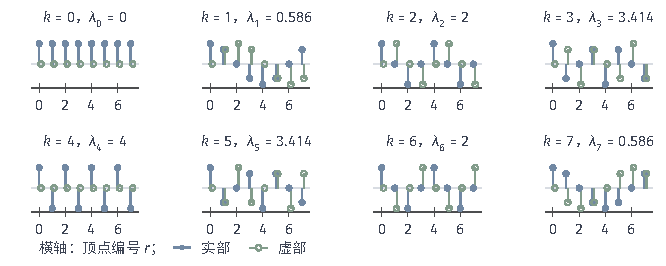
\includegraphics[width=112mm]{figures/01-basic-mathematics/04-graphs/tikz/c6-cycle-fourier-basis/figure.pdf}
  \caption{八点单位权环的复指数特征向量$u_k[r]=\mathrm e^{2\pi\mathrm ikr/8}/\sqrt8$。蓝色实心为实部，绿色空心为虚部，横轴为顶点编号$r$，标题给出特征值$\lambda_k=2-2\cos(2\pi k/8)$。$k$与$8-k$的实部相同、虚部相反，特征值相等；按$k$排列时特征值先增后减，$k=4$的振荡最快。}
  \label{fig:graph-spec-cycle-fourier-basis}
\end{figure}

图~\ref{fig:graph-spec-cycle-fourier-basis}画出$N=8$时的全部八个特征向量。编号$k$是复振荡沿环转动的圈数，不是特征值的次序：特征值随$k$先增后减，$k$与$N-k$给出相同的特征值。原因是$\bm u_{N-k}=\overline{\bm u_k}$，二者沿相反方向转动，相邻顶点间的差异一样大。

\paragraph{四点环上的单位脉冲}
取$N=4$，此时$u_k[r]=\tfrac12\mathrm i^{kr}$，特征值依次为$\lambda_0=0$、$\lambda_1=2$、$\lambda_2=4$、$\lambda_3=2$，其中$\lambda_1=\lambda_3$是一对重复特征值。对顶点$0$上的单位脉冲$\bm f=\bm e_0$，
\[
 \widehat f_k=\sum_r\overline{u_k[r]}f[r]=\overline{u_k[0]}=\tfrac12,\qquad k=0,1,2,3 ,
\]
四个谱坐标都是$\tfrac12$。重构时，$f[r]=\sum_k\tfrac12\cdot\tfrac12\mathrm i^{kr}=\tfrac14\sum_{k=0}^3\mathrm i^{kr}$：$r=0$时为$1$；$r=1,2,3$时公比$\mathrm i^r\neq1$且$(\mathrm i^r)^4=1$，几何和为零。于是恢复了$\bm e_0$。若把脉冲移到顶点$1$，谱坐标变为$\overline{u_k[1]}=\tfrac12\mathrm i^{-k}$，即$\tfrac12,-\tfrac{\mathrm i}2,-\tfrac12,\tfrac{\mathrm i}2$：模都不变，只是辐角随$k$转动。沿环平移只改变各谱坐标的相位，这正是复指数基在环上的方便之处。

这组复指数与信号处理中离散傅里叶变换使用的振荡是同一组，只差归一化常数$\sqrt N$。完整的离散傅里叶变换及其快速算法由后续信号部分展开。环的特殊之处在于存在把每个顶点移到下一个顶点的平移，复指数正是在平移下只改变相位的函数；一般图没有这样的平移，按顶点编号对数组做快速傅里叶变换，得不到该图拉普拉斯的谱坐标。

% 第6章第6节：图滤波（滤波问题与谱响应、基于谱分解的滤波、多项式滤波与局部计算、方法比较与结果检验）。

\section{图滤波}
\label{sec:graph-filtering}

图傅里叶变换只换坐标，不改变函数。本节转向改变函数：规定每个模态保留多少、衰减多少，得到新的顶点函数。先定义滤波的目标，再比较两种实现：一种先求谱基再逐模态缩放，另一种只用拉普拉斯的稀疏乘法。若目标响应在图谱上恰好可以由所用多项式表示，两种实现给出同一个输出；若只是用多项式近似，就需要控制输出误差。

\subsection{滤波问题与谱响应}
\label{sec:graph-spec-filtering-problem}

传感器读数常混有逐点跳动的噪声，而真实的温度场在相邻测点间变化平缓。上一节的分解~\eqref{eq:graph-spec-parseval}说明，逐点跳动主要落在大特征值的模态上。于是“去噪”可以表述为：保留小特征值的模态，压低大特征值的模态。把每个模态保留的比例写成特征值的函数，就得到下面的定义。

\begin{definition}[谱滤波]
\label{def:graph-spec-spectral-filter}
给定图算子$\bm L=\bm U\bm\Lambda\bm U^{\top}$、输入$\bm f$和定义在全部特征值上的实函数$g$，称
\begin{equation}
 \bm y=g(\bm L)\bm f=\bm U\,g(\bm\Lambda)\,\bm U^{\top}\bm f,\qquad
 g(\bm\Lambda)=\operatorname{diag}\bigl(g(\lambda_1),\ldots,g(\lambda_n)\bigr)
 \label{eq:graph-spec-spectral-filter}
\end{equation}
为$\bm f$经\term{谱响应}（spectral response）$g$的\term{图滤波}（graph filtering）输出。按谱坐标写，$\widehat y_k=g(\lambda_k)\widehat f_k$。
\end{definition}

$g(\bm L)$正是第~\ref{sec:ls-matrix-functions}节沿特征方向定义的矩阵函数。几种典型响应各有含义：$g\equiv1$时$\bm y=\bm f$，原样输出；$g(0)=1$保证零模不变，在正权支撑连通时就是保持各点的平均值；$g$随$\lambda$递减到接近零，则高频模态被压低，输出比输入平缓，这样的响应称为低通。这里规定的是要得到什么输出，下面两小节讨论怎样算出它。

\paragraph{定义的合理性}
$\bm U$不唯一，需要确认输出不依赖它的选取。式~\eqref{eq:graph-spec-spectral-filter}对同一特征值的各个模态使用同一个数$g(\lambda)$，所以$g(\bm L)=\sum_\lambda g(\lambda)\bm P_\lambda$，其中$\bm P_\lambda$是到特征空间的正交投影，只由$\bm L$决定（第~\ref{sec:ls-matrix-functions}节）。重编号也不改变结果：$\bm P\bm L\bm P^{\top}$的特征向量是$\bm P\bm u_k$，特征值不变，于是$g(\bm P\bm L\bm P^{\top})=\bm Pg(\bm L)\bm P^{\top}$，对重排后的输入$\bm P\bm f$输出$\bm P\bm y$，即输出随顶点一起重排。

\paragraph{放大界}
滤波可能把函数放大，放大多少由响应的最大幅度控制。由式~\eqref{eq:graph-spec-parseval}，
\begin{equation}
 \begin{gathered}
 \lVert\bm y\rVert_2^2=\sum_kg(\lambda_k)^2\widehat f_k^{\,2}\leq\Bigl(\max_k|g(\lambda_k)|\Bigr)^2\lVert\bm f\rVert_2^2,\\
 \bm y^{\top}\bm L\bm y=\sum_k\lambda_kg(\lambda_k)^2\widehat f_k^{\,2}\leq\Bigl(\max_k|g(\lambda_k)|\Bigr)^2\bm f^{\top}\bm L\bm f .
 \end{gathered}
 \label{eq:graph-spec-filter-bound}
\end{equation}
所以只要在全部特征值上$|g(\lambda_k)|\leq1$，输出的幅值和沿边变化能量都不会超过输入。没有这个条件，就不能断言滤波不增加幅值或能量；例如$g(\lambda)=1+\lambda$会放大高频模态。

\subsection{基于谱分解的滤波}
\label{sec:graph-spec-eigendecomposition-filter}

最直接的实现照搬定义：先求谱基，再在谱坐标中逐个缩放。

\begin{algorithm}[基于谱分解的图滤波]
\label{alg:graph-spec-eigendecomposition-filter}
输入：$n\times n$实对称图算子$\bm L$，顶点函数$\bm f$，谱响应$g$。输出：$\bm y=g(\bm L)\bm f$。
\begin{enumerate}
 \item 求谱分解$\bm L=\bm U\bm\Lambda\bm U^{\top}$（同一个$\bm L$只需做一次）。
 \item 投影：$\widehat{\bm f}=\bm U^{\top}\bm f$。
 \item 逐模态缩放：$\widehat y_k=g(\lambda_k)\widehat f_k$，$k=1,\ldots,n$。
 \item 重构：$\bm y=\bm U\widehat{\bm y}$。
\end{enumerate}
\end{algorithm}

三步合起来是$\bm U g(\bm\Lambda)\bm U^{\top}\bm f$，正确性直接来自定义。开销要分开计：第1步对稠密矩阵通常需要$O(n^3)$次运算，存储$\bm U$需要$O(n^2)$空间；第2、4步各是一次稠密矩阵乘向量，第3步计算$n$个响应值，合计每个输入$O(n^2)$。图算子固定、要处理许多个输入时，第1步的结果可以反复使用，摊到每个输入上的代价随之下降。若为节省开销只求前若干个模态、把其余模态的响应当作零，就改变了目标响应，实际计算的是另一种截断滤波，需要另行说明误差，不能仍称为原响应的精确实现。

\paragraph{三点路径上的低通滤波}
在单位权三点路径上取$\bm f=(3,1,2)^{\top}$与响应$g(\lambda)=1/(1+\lambda)$。上一节已求出谱坐标$\widehat{\bm f}=(2\sqrt3,\tfrac1{\sqrt2},\tfrac{\sqrt6}2)^{\top}$，三个特征值$0,1,3$的响应为$1,\tfrac12,\tfrac14$，所以
\[
 \bm y=2\sqrt3\,\bm u_1+\tfrac12\cdot\tfrac1{\sqrt2}\,\bm u_2+\tfrac14\cdot\tfrac{\sqrt6}2\,\bm u_3
 =\begin{bmatrix}2\\2\\2\end{bmatrix}+\frac14\begin{bmatrix}1\\0\\-1\end{bmatrix}+\frac18\begin{bmatrix}1\\-2\\1\end{bmatrix}
 =\begin{bmatrix}19/8\\7/4\\15/8\end{bmatrix}.
\]
常量成分$(2,2,2)^{\top}$原样保留，所以输出各分量之和仍为$6$；两个变化成分分别缩小为原来的$\tfrac12$和$\tfrac14$。输出的能量为$(\tfrac58)^2+(\tfrac18)^2=\tfrac{13}{32}\approx0.41$，远小于输入的$5$。这个响应恰好对应求解线性方程组：$g(\bm L)=(\bm I+\bm L)^{-1}$，可以直接核对$(\bm I+\bm L)\bm y=\bm f$。

\subsection{多项式滤波与局部计算}
\label{sec:graph-spec-polynomial-filter}

谱分解的代价主要花在求$\bm U$上。若响应是多项式，可以完全绕开特征向量。设$g(\lambda)=\sum_{r=0}^K\alpha_r\lambda^r$，由$\bm L^r=\bm U\bm\Lambda^r\bm U^{\top}$，
\begin{equation}
 g(\bm L)\bm f=\sum_{r=0}^K\alpha_r\bm L^r\bm f ,
 \label{eq:graph-spec-polynomial-filter}
\end{equation}
右端只需要反复用$\bm L$乘向量。按这种方式计算谱滤波称为\term{多项式图滤波}（polynomial graph filtering）。

\begin{algorithm}[多项式图滤波]
\label{alg:graph-spec-polynomial-filter}
输入：以正权边邻接表存储的$\bm L$，顶点函数$\bm f$，系数$\alpha_0,\ldots,\alpha_K$。输出：$\bm y=\sum_r\alpha_r\bm L^r\bm f$。状态：当前幂次向量$\bm v^{(r)}=\bm L^r\bm f$与累加向量$\bm y$。
\begin{enumerate}
 \item 置$\bm v^{(0)}=\bm f$，$\bm y=\alpha_0\bm f$。
 \item 对$r=1,\ldots,K$：从完整的旧向量$\bm v^{(r-1)}$读取，按$(\bm L\bm v)_i=d_iv_i-\sum_jw_{i,j}v_j$把结果写入另一个缓冲区，得到$\bm v^{(r)}$；再令$\bm y\leftarrow\bm y+\alpha_r\bm v^{(r)}$。
\end{enumerate}
\end{algorithm}

第2步必须同步读取旧向量，理由与第~\ref{sec:graph-spec-neighborhood-aggregation}小节相同：就地改写会让后面的顶点读到本轮的新值，算出的就不再是$\bm L\bm v$。按归纳，每轮结束时$\bm v^{(r)}=\bm L^r\bm f$，$\bm y$累加了前$r$项，所以算法输出式~\eqref{eq:graph-spec-polynomial-filter}。

\paragraph{依赖范围}
多项式滤波的输出只依赖附近的顶点。一次乘法中，$(\bm L\bm v)_i$只读取$v_i$与正权邻居的值。归纳可得，$(\bm L^r\bm v)_i$只依赖在正权支撑图中与$i$相距至多$r$步的顶点：第$r$轮读取的邻居值本身只依赖再远$r-1$步以内的顶点。所以$K$次多项式滤波在顶点$i$的输出，只依赖$i$的$K$跳邻域。

这是范围的上界，不是说范围内的每个顶点都一定产生非零贡献。单位权三点路径上，$(\bm L^2-3\bm L)\bm e_1=(2,-3,1)^{\top}-3(1,-1,0)^{\top}=(-1,0,1)^{\top}$：顶点$2$与顶点$1$只隔一条边，但两项贡献恰好相消，输出为零。

\begin{figure}[!htb]
  \centering
  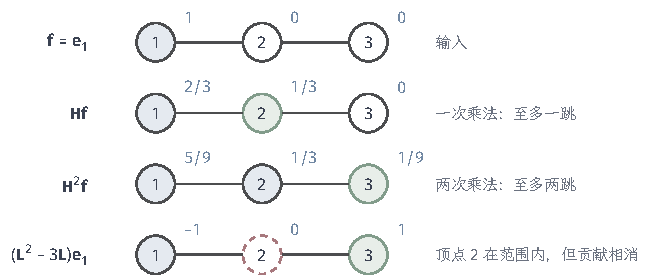
\includegraphics[width=110mm]{figures/01-basic-mathematics/04-graphs/tikz/c6-polynomial-locality/figure.pdf}
  \caption{单位权三点路径上多项式滤波的依赖范围，$\bm H=\bm I-\bm L/3$，蓝色数字为各顶点的输出。从$\bm f=\bm e_1$出发，一次作用只到达一跳邻居（绿色），两次作用才到达两跳外的顶点$3$。最后一行$(\bm L^2-3\bm L)\bm e_1$中，顶点$2$位于范围内，但贡献相消为零（红色虚线）。}
  \label{fig:graph-spec-polynomial-locality}
\end{figure}

图~\ref{fig:graph-spec-polynomial-locality}用一次多项式$\bm H=\bm I-\bm L/3$展示范围怎样扩大。从$\bm e_1$出发，
\[
 \bm H\bm e_1=\bm e_1-\tfrac13(1,-1,0)^{\top}=\bigl(\tfrac23,\tfrac13,0\bigr)^{\top},\qquad
 \bm H^2\bm e_1=\bigl(\tfrac59,\tfrac13,\tfrac19\bigr)^{\top}.
\]
第一轮只有顶点$1$、$2$非零，第二轮才到达顶点$3$。从谱的角度看，$\bm H$的响应$1-\lambda/3$在特征值$0,1,3$上取$1,\tfrac23,0$：常量模态保留，最高频模态被完全消去。

\paragraph{开销与近似误差}
以邻接表存储正权边，一次$\bm L$乘向量要访问每个顶点和每条正权边常数次，需要$O(n+m_+)$次运算；$K$轮共$O(K(n+m_+))$。除了图本身，只需保存旧向量、新向量和累加向量，额外空间为$O(n)$。整个过程不求任何特征向量。

多项式能表示的响应有限，一般的响应$g$只能近似。设多项式$p$在一个包含全部特征值的区间上满足$|g(\lambda)-p(\lambda)|\leq\varepsilon$。对差$g-p$使用放大界~\eqref{eq:graph-spec-filter-bound}，得
\[
 \lVert g(\bm L)\bm f-p(\bm L)\bm f\rVert_2\leq\varepsilon\lVert\bm f\rVert_2 .
\]
所以只要知道谱落在哪个区间，就能把标量函数的逼近误差转成输出误差。对$\bm L_{\mathrm{sym}}$，定理~\ref{thm:graph-spec-normalized-bound}给出区间$[0,2]$；对$\bm L$可用$[0,2d_{\max}]$。图~\ref{fig:graph-spec-filter-responses}(b)在$[0,2]$上逼近低通响应$1/(1+3\lambda)$：用Chebyshev节点插值，$K=2$时最大误差约$0.18$，$K=4$时约$0.038$。

\begin{figure}[!htb]
  \centering
  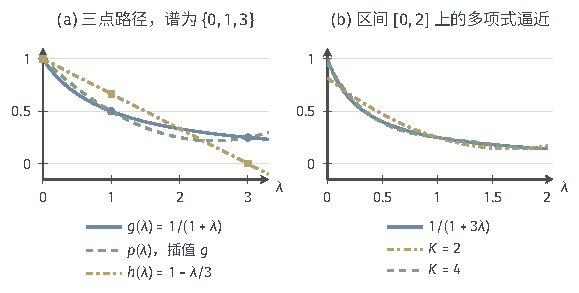
\includegraphics[width=98mm]{figures/01-basic-mathematics/04-graphs/tikz/c6-filter-responses/figure.pdf}
  \caption{谱响应与多项式。(a)~三点路径的谱为$\{0,1,3\}$：蓝色为目标$g(\lambda)=1/(1+\lambda)$，绿色虚线为在三个特征值上与$g$相等的二次多项式$p(\lambda)=1-\tfrac58\lambda+\tfrac18\lambda^2$，二者只在圆点处重合；黄色点划线为$h(\lambda)=1-\lambda/3$，方点是它在特征值上的取值。(b)~区间$[0,2]$上目标$1/(1+3\lambda)$及其$K=2$、$K=4$次Chebyshev节点插值，最大误差约为$0.18$和$0.038$。}
  \label{fig:graph-spec-filter-responses}
\end{figure}

另一种情形是已知全部互不相同的特征值。一个有限集合上的任意函数都可以用插值多项式精确匹配，$s$个不同的特征值需要至多$s-1$次。三点路径的谱为$\{0,1,3\}$，取$p(\lambda)=1-\tfrac58\lambda+\tfrac18\lambda^2$，直接代入得$p(0)=1$、$p(1)=\tfrac12$、$p(3)=\tfrac14$，与$g(\lambda)=1/(1+\lambda)$在三个特征值上相同。于是$p(\bm L)=g(\bm L)$，尽管$p$与$g$作为函数并不相同，见图~\ref{fig:graph-spec-filter-responses}(a)。这种精确匹配要求事先知道特征值，在大图上通常做不到。

\subsection{方法比较与结果检验}
\label{sec:graph-spec-filter-comparison}

比较两种实现时，要固定同一个图算子、同一个输入和同一个目标响应，只比较计算方式。表~\ref{tab:graph-spec-filter-comparison}列出主要差别。

\begin{table}[!htb]
  \centering\small
  \begin{tabularx}{\linewidth}{@{}lXX@{}}
    \toprule
    & 基于谱分解（算法~\ref{alg:graph-spec-eigendecomposition-filter}） & 多项式滤波（算法~\ref{alg:graph-spec-polynomial-filter}）\\
    \midrule
    预处理 & 稠密特征分解，$O(n^3)$ & 无；逼近一般响应时需要谱区间 \\
    单个输入 & $O(n^2)$ & $O(K(n+m_+))$ \\
    额外存储 & $\bm U$，$O(n^2)$ & 三个向量，$O(n)$ \\
    适用响应 & 任意$g$，精确 & 多项式精确；一般$g$有误差$\varepsilon\lVert\bm f\rVert_2$ \\
    \bottomrule
  \end{tabularx}
  \caption{同一图算子、输入和目标响应下两种滤波实现的比较。$n$为顶点数，$m_+$为正权边数，$K$为多项式次数。}
  \label{tab:graph-spec-filter-comparison}
\end{table}

多项式响应可以用两种方法实现同一个算子，结果相同；用多项式逼近一般响应，则在实现方式之外又改变了目标，多出一项近似误差。这两种差别要分开说明，不能把“实现方式不同”和“目标响应不同”混为一谈。

\paragraph{交叉核对}
在小图上，可以用两种实现互相核对。仍取三点路径、$\bm f=(3,1,2)^{\top}$，用插值多项式$p$按算法~\ref{alg:graph-spec-polynomial-filter}计算：$\bm L\bm f=(2,-3,1)^{\top}$，$\bm L^2\bm f=(5,-9,4)^{\top}$，
\[
 p(\bm L)\bm f=\bm f-\tfrac58\bm L\bm f+\tfrac18\bm L^2\bm f
 =\Bigl(3-\tfrac{10}8+\tfrac58,\ 1+\tfrac{15}8-\tfrac98,\ 2-\tfrac58+\tfrac48\Bigr)^{\top}
 =\Bigl(\tfrac{19}8,\tfrac74,\tfrac{15}8\Bigr)^{\top},
\]
与谱分解的结果完全一致，而这次计算没有用到任何特征向量。还可以检查几项必然成立的性质：$\max_k|g(\lambda_k)|=1$，按放大界应有$\lVert\bm y\rVert_2^2\leq\lVert\bm f\rVert_2^2$，实际为$\tfrac{782}{64}\approx12.2\leq14$；$g(0)=1$且图连通，各分量之和应保持为$6$；把顶点重编号后重算，输出应随之重排。

本节的滤波只依赖有限维谱分解，没有引入时间。连续的热扩散及其时间离散会给出特定的响应族，它们在后续过程与信号部分建立。

% 第6章第7节：谱划分（图划分问题与割的表示、RatioCut谱方法、NCut谱方法）。

\section{谱划分}
\label{sec:graph-spectral-partition}

最后回到章首的第三个问题：按连接强弱把顶点分成两组。本节固定$n\geq2$，要求两组都非空。先用指示向量把跨组边权写成拉普拉斯的二次型，说明只最小化跨组边权为什么会得到失衡的划分；再分别按顶点数和连接体积引入平衡，把离散问题写成Rayleigh商，放宽取值限制后用谱展开求解。连续解给出下界和候选分组，但它本身不是分组，二者要始终分开。

\subsection{图划分问题与割的表示}
\label{sec:graph-spec-partition-problem}

把顶点集分成$S$与$\bar S=V\setminus S$两组，跨组的连接强度用
\[
 \operatorname{cut}(S,\bar S)=\sum_{i\in S}\sum_{j\in\bar S}w_{i,j}
\]
衡量。这沿用了第~\ref{sec:graph-max-flow}节割的想法：把顶点分到两侧，累计跨过两侧的边上的数值。区别在于这里的图是无向的，没有源和汇，两个方向不加区分。

割权可以写成二次型。令$\bm s$为$S$的指示向量，$s_i=1$（$i\in S$）或$0$（$i\in\bar S$）。代入能量式~\eqref{eq:graph-spec-dirichlet-energy}，两端在同一组的边$(s_i-s_j)^2=0$，跨组的边$(s_i-s_j)^2=1$，所以
\begin{equation}
 \bm s^{\top}\bm L\bm s=\sum_{\{i,j\}\in E}w_{i,j}(s_i-s_j)^2=\operatorname{cut}(S,\bar S).
 \label{eq:graph-spec-cut-quadratic}
\end{equation}
于是划分问题变成在取值为$0$或$1$的向量上最小化$\bm L$的二次型。

只最小化割权并不够。若允许空组，$S=\varnothing$的割权为零，问题平凡；这正是要求两组非空的原因。即使要求非空，最小割也常常只切下一个连接很弱的顶点。图~\ref{fig:graph-spec-cut-indicator}中两个单位权三角形由一条单位权边相连，顶点$7$以权$0.6$挂在顶点$2$上。直观的分法是沿中间的桥切开，割权为$1$；但只切下顶点$7$的割权是$0.6$，枚举全部$63$种非空二分可知它就是最小割。单纯的割权不关心两组各有多大。

\begin{figure}[!htb]
  \centering
  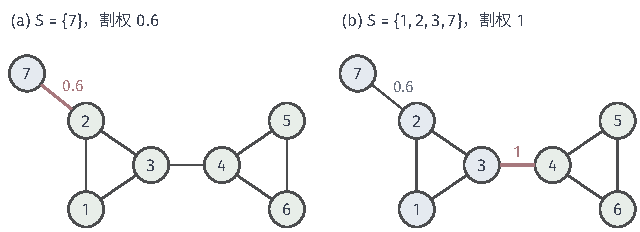
\includegraphics[width=108mm]{figures/01-basic-mathematics/04-graphs/tikz/c6-cut-indicator/figure.pdf}
  \caption{割与指示向量。两个单位权三角形由桥$\{3,4\}$相连，顶点$7$以权$0.6$连到顶点$2$。蓝色顶点属于$S$（指示向量取$1$），绿色顶点属于$\bar S$（取$0$），红色边跨组，$\bm s^{\top}\bm L\bm s$等于红色边权之和。(a)~$S=\{7\}$，割权$0.6$，是全部非空二分中的最小割；(b)~$S=\{1,2,3,7\}$，割权$1$，两组大小相近。}
  \label{fig:graph-spec-cut-indicator}
\end{figure}

\paragraph{松弛给出的上下界}
下面两小节都采用同一种论证，这里先把逻辑说清。设离散问题在有限可行集$\mathcal F$上最小化目标$J$，最优值为$J^\star$。若把可行集扩大为$\mathcal C\supseteq\mathcal F$，并把$J$延拓到$\mathcal C$上，可选的对象只多不少，最小值只能下降：$L=\min_{\mathcal C}J\leq J^\star$。这种做法称为\term{连续松弛}（continuous relaxation），它给出下界。另一方面，从连续解出发构造任意一个合法分组并计算原目标值$U$，则$U\geq J^\star$，它给出上界。于是
\[
 0\leq U-J^\star\leq U-L ,
\]
差$U-L$限制了所得分组可能的次优程度。它只是次优程度的上界，只有下界恰好取到$J^\star$时才等于真实的差距。

\subsection{RatioCut谱方法}
\label{sec:graph-spec-ratio-cut}

为了不让一组过小，把割权按两组的顶点数放大。设$a=|S|>0$，$b=|\bar S|>0$，定义\term{比率割}（RatioCut）
\begin{equation}
 \operatorname{RatioCut}(S,\bar S)=\operatorname{cut}(S,\bar S)\Bigl(\frac1a+\frac1b\Bigr).
 \label{eq:graph-spec-ratio-cut}
\end{equation}
一组越小，$\frac1a$越大，切下它的代价就越高。在图~\ref{fig:graph-spec-cut-indicator}中，只切下顶点$7$的RatioCut为$0.6\cdot(1+\tfrac16)=0.7$，沿桥切开的RatioCut为$1\cdot(\tfrac14+\tfrac13)=\tfrac7{12}\approx0.58$；枚举可知后者是全部非空二分中的最小值。

\paragraph{两水平向量}
接下来把RatioCut写成Rayleigh商。对给定分组构造在两组上分别取常数的向量
\begin{equation}
 f_i=\sqrt{b/a}\quad(i\in S),\qquad f_i=-\sqrt{a/b}\quad(i\in\bar S).
 \label{eq:graph-spec-ratio-cut-vector}
\end{equation}
逐项计算：$\bm1^{\top}\bm f=a\sqrt{b/a}-b\sqrt{a/b}=\sqrt{ab}-\sqrt{ab}=0$；$\bm f^{\top}\bm f=a\cdot\tfrac ba+b\cdot\tfrac ab=n$；跨组边上的差都是$\sqrt{b/a}+\sqrt{a/b}=n/\sqrt{ab}$，同组边上的差为零，所以
\[
 \bm f^{\top}\bm L\bm f=\operatorname{cut}(S,\bar S)\frac{n^2}{ab}=n\operatorname{cut}(S,\bar S)\Bigl(\frac1a+\frac1b\Bigr)=n\operatorname{RatioCut}(S,\bar S).
\]
因此$\operatorname{RatioCut}(S,\bar S)=\bm f^{\top}\bm L\bm f/\bm f^{\top}\bm f$。最小化RatioCut，等价于在“与$\bm1$正交、只取两个由分组决定的值”的向量中最小化$\bm L$的Rayleigh商。去掉“只取两个值”的限制，只保留$\bm f\neq\bm0$与$\bm f\perp\bm1$，可行集从有限个向量扩大为一个$n-1$维子空间去掉原点，这就是连续松弛。

\begin{theorem}[RatioCut的谱下界]
\label{thm:graph-spec-ratio-cut-bound}
设$\bm L$的特征值为$0=\lambda_1\leq\lambda_2\leq\cdots\leq\lambda_n$，则
\[
 \min_{\bm f\neq\bm0,\ \bm f\perp\bm1}\frac{\bm f^{\top}\bm L\bm f}{\bm f^{\top}\bm f}=\lambda_2 ,
\]
最小值在第二特征向量$\bm u_2$处取到。因此对每个非空二分都有$\operatorname{RatioCut}(S,\bar S)\geq\lambda_2$。
\end{theorem}

\begin{proof}
$\bm1$在$\bm L$的零空间中，所以可以取标准正交特征基使$\bm u_1=\bm1/\sqrt n$。$\bm f\perp\bm1$意味着$\bm f$在$\bm u_1$上的坐标为零，$\bm f=\sum_{k\geq2}c_k\bm u_k$。由式~\eqref{eq:graph-spec-parseval}，
\[
 \frac{\bm f^{\top}\bm L\bm f}{\bm f^{\top}\bm f}=\frac{\sum_{k\geq2}\lambda_kc_k^2}{\sum_{k\geq2}c_k^2},
\]
它是$\lambda_2,\ldots,\lambda_n$以$c_k^2$为权的加权平均，不小于$\lambda_2$；取$\bm f=\bm u_2$时等于$\lambda_2$。每个两水平向量~\eqref{eq:graph-spec-ratio-cut-vector}都在可行集中，所以RatioCut不小于这个最小值。
\end{proof}

证明只用到已有的谱分解，不需要拉格朗日乘子或一般的约束优化理论。第二特征向量常称为Fiedler向量；正权支撑图连通时，由定理~\ref{thm:graph-spec-null-space}知$\lambda_2>0$。

\paragraph{从谱方向恢复分组}
连续最优解$\bm u_2$一般不是两水平向量，需要把它变回分组。既然两水平向量在$S$上取正值、在$\bar S$上取负值，自然的做法是按$\bm u_2$的坐标排序，在某个位置切开。

\begin{algorithm}[谱划分的阈值扫描]
\label{alg:graph-spec-sweep}
输入：图与谱方向$\bm v$（RatioCut用$\bm u_2$）。输出：一个非空二分及其原目标值$U$。
\begin{enumerate}
 \item 按$\bm v$的坐标从大到小排列顶点；坐标相同的顶点视为一个整体。
 \item 在相邻两个不同坐标值之间依次设阈值，坐标大于阈值的顶点组成$S$，其余组成$\bar S$，两组都非空。
 \item 对每个候选分组，用原目标（RatioCut或NCut）计算其值，保留最小者作为$U$。
\end{enumerate}
\end{algorithm}

这种逐个阈值试探的做法称为\term{阈值扫描}（threshold sweep）。扫描时不必每次重算割权：把顶点$i$从$\bar S$移入$S$时，它连向$S$的边不再跨组，连向$\bar S$的边开始跨组，所以割权增加$\sum_{j\in\bar S}w_{i,j}-\sum_{j\in S}w_{i,j}$，只需访问$i$的邻边。组大小或体积同样可以逐步更新。

\begin{figure}[!htb]
  \centering
  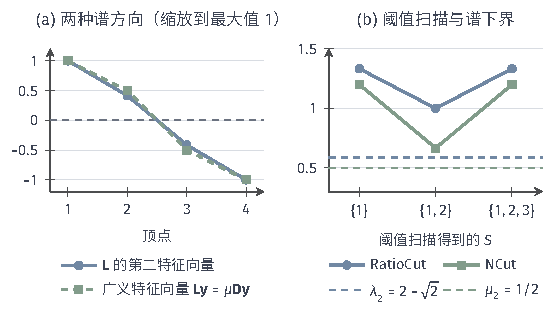
\includegraphics[width=94mm]{figures/01-basic-mathematics/04-graphs/tikz/c6-four-path-sweep/figure.pdf}
  \caption{单位权四点路径$1-2-3-4$上的两种谱划分。(a)~$\bm L$的第二特征向量（蓝）与广义特征问题$\bm L\bm y=\mu\bm D\bm y$的第二特征向量（绿），均按最大绝对值缩放到$1$；二者在零点两侧给出同样的分组，但中间两点的相对幅度不同。(b)~按坐标排序扫描三个阈值得到的原目标值，实线为RatioCut与NCut，虚线为相应谱下界$\lambda_2=2-\sqrt2$与$\mu_2=\tfrac12$；两种目标都在$S=\{1,2\}$处最小，且严格高于下界。}
  \label{fig:graph-spec-four-path-sweep}
\end{figure}

\paragraph{四点路径算例}
取单位权四点路径$1-2-3-4$。它的拉普拉斯的特征值为$0$、$2-\sqrt2$、$2$、$2+\sqrt2$，第二特征向量正比于$(1+\sqrt2,1,-1,-1-\sqrt2)^{\top}$；可以直接核对$\bm L\bm v=(2-\sqrt2)\bm v$。按坐标扫描得到三个候选分组，RatioCut依次为
\[
 S=\{1\}:\ 1\cdot\bigl(1+\tfrac13\bigr)=\tfrac43,\qquad
 S=\{1,2\}:\ 1\cdot\bigl(\tfrac12+\tfrac12\bigr)=1,\qquad
 S=\{1,2,3\}:\ \tfrac43 ,
\]
所以$U=1$。枚举全部七种非空二分，离散最优值也是$1$，在$\{1,2\}|\{3,4\}$处取到。谱下界为$\lambda_2=2-\sqrt2\approx0.586$，严格小于$1$，见图~\ref{fig:graph-spec-four-path-sweep}。这说明松弛通常不紧：这里恢复的分组恰好最优，但只凭$U-L\approx0.414$并不能确认这一点。

\paragraph{开销}
整个方法的开销分三部分。求$\bm u_2$：稠密完整特征分解需要$O(n^3)$时间、$O(n^2)$空间；大型稀疏图常用只求少数特征向量的迭代方法，其代价取决于求解器、所需精度和$\lambda_2$与$\lambda_3$的间隔，不能只因为$\bm L$稀疏就断言是线性时间。排序需要$O(n\log n)$。扫描时每个顶点移动一次，每条正权边被访问常数次，需要$O(n+m_+)$。

\subsection{NCut谱方法}
\label{sec:graph-spec-normalized-cut}

RatioCut用顶点个数衡量组的大小。另一种选择是用组内的连接总量：一组顶点的加权度之和
\[
 \operatorname{vol}(S)=\sum_{i\in S}d_i
\]
称为它的\term{体积}（volume）。设$p=\operatorname{vol}(S)>0$，$q=\operatorname{vol}(\bar S)>0$，定义\term{归一化割}（normalized cut，NCut）
\begin{equation}
 \operatorname{NCut}(S,\bar S)=\operatorname{cut}(S,\bar S)\Bigl(\frac1p+\frac1q\Bigr).
 \label{eq:graph-spec-normalized-cut}
\end{equation}
它要求两组的体积都为正。在图~\ref{fig:graph-spec-cut-indicator}中，顶点$7$的体积只有$0.6$，只切下它的NCut约为$1.04$；沿桥切开时两侧体积为$8.2$与$7$，NCut为$\tfrac1{8.2}+\tfrac17\approx0.26$，是全部非空二分中的最小值。

\paragraph{度加权的两水平向量}
与RatioCut平行，构造$y_i=\sqrt{q/p}$（$i\in S$）、$y_i=-\sqrt{p/q}$（$i\in\bar S$）。这次用度加权核对：
\[
 \bm y^{\top}\bm D\bm1=p\sqrt{q/p}-q\sqrt{p/q}=0,\qquad
 \bm y^{\top}\bm D\bm y=p\cdot\tfrac qp+q\cdot\tfrac pq=\operatorname{vol}(V),
\]
跨组边上的差为$\sqrt{q/p}+\sqrt{p/q}=(p+q)/\sqrt{pq}$，所以$\bm y^{\top}\bm L\bm y=\operatorname{cut}(S,\bar S)(p+q)^2/(pq)=\operatorname{vol}(V)\operatorname{NCut}(S,\bar S)$。于是
\[
 \operatorname{NCut}(S,\bar S)=\frac{\bm y^{\top}\bm L\bm y}{\bm y^{\top}\bm D\bm y},\qquad \bm y^{\top}\bm D\bm1=0 .
\]
与RatioCut相比，正交条件和长度都换成了度加权的版本，这正是第~\ref{sec:graph-spec-degree-inner-product}小节的度加权内积。两种方法采用了不同的平衡尺度。

\paragraph{化为对称归一化拉普拉斯}
先把谱计算限制在正度顶点$V_+$上。支撑孤点的体积为零，会让$\bm D$奇异，还会给$\bm L_{\mathrm{sym}}$带来额外的零特征向量$\bm e_v$，它们对应的并不是合法的正体积分组；孤点的处理放在下面单独说明。在$V_+$上$\bm D$正定，作坐标代换$\bm x=\bm D^{1/2}\bm y$，则
\[
 \frac{\bm y^{\top}\bm L\bm y}{\bm y^{\top}\bm D\bm y}=\frac{\bm x^{\top}\bm L_{\mathrm{sym}}\bm x}{\bm x^{\top}\bm x},\qquad
 \bm y^{\top}\bm D\bm1=\bm x^{\top}\bm D^{1/2}\bm1=0 .
\]
约束变成$\bm x\perp\bm D^{1/2}\bm1$，而$\bm D^{1/2}\bm1$正是$\bm L_{\mathrm{sym}}$的零特征向量（第~\ref{sec:graph-spec-null-space-components}小节）。取$\bm L_{\mathrm{sym}}$的标准正交特征基，使第一个向量为$\bm D^{1/2}\bm1/\lVert\bm D^{1/2}\bm1\rVert_2$，重复定理~\ref{thm:graph-spec-ratio-cut-bound}的证明，可知松弛问题的最小值是$\bm L_{\mathrm{sym}}$的第二小特征值$\mu_2$，在相应特征向量$\bm x_2$处取到，并且每个合法分组都有$\operatorname{NCut}\geq\mu_2$。

换回原坐标$\bm y_2=\bm D^{-1/2}\bm x_2$，由$\bm L_{\mathrm{sym}}\bm x_2=\mu_2\bm x_2$左乘$\bm D^{1/2}$得
\[
 \bm L\bm y_2=\mu_2\bm D\bm y_2 ,
\]
这是一个广义特征问题（定义~\ref{def:matrix-analysis-generalized-eigenvalue}），也可写成$\bm L_{\mathrm{rw}}\bm y_2=\mu_2\bm y_2$。阈值扫描应当使用$\bm y_2$的坐标。一般的非正则图上，不能用组合拉普拉斯的第二特征向量代替它：只有每个顶点度都等于同一个$d$时，$\bm L_{\mathrm{sym}}=\bm L/d$，两种方向才相同，特征值相差因子$d$。

\paragraph{分量、孤点与合法性}
若正度顶点组成多个正权支撑分量，每个分量的体积都为正，把其中一部分分量放进$S$、其余放进$\bar S$，割权为零，NCut为零，已经最优。此时$\mu_2=0$，零特征空间是多维的，其中任意一个向量都是“第二特征向量”，应直接按分量分组，分量可以由第~\ref{sec:graph-connectivity-computation}节的遍历求出。支撑孤点不影响割权，也不影响体积，求出正度部分的分组后可以把它们放进任一组。若$E_+$为空，所有顶点的体积都是零，当前NCut问题没有合法的二分；只要有一条正权边，把它的两个端点分到两侧就得到两个正体积组。所以恢复时要检查两组非空且体积为正，再重新计算原NCut。

\paragraph{四点路径上的对照}
回到单位权四点路径，$\bm D=\operatorname{diag}(1,2,2,1)$。广义特征问题的第二特征值为$\mu_2=\tfrac12$，特征向量正比于$\bm y_2=(1,\tfrac12,-\tfrac12,-1)^{\top}$；直接核对$\bm L\bm y_2=(\tfrac12,\tfrac12,-\tfrac12,-\tfrac12)^{\top}=\tfrac12\bm D\bm y_2$。扫描得到的NCut依次为$\tfrac65$、$\tfrac23$、$\tfrac65$，枚举全部七种二分可知离散最优值为$\tfrac23$，同样在$\{1,2\}|\{3,4\}$处取到，严格高于下界$\tfrac12$。与RatioCut比较，图~\ref{fig:graph-spec-four-path-sweep}显示两种谱方向在中间两点的相对幅度不同（$\tfrac1{1+\sqrt2}\approx0.41$对$\tfrac12$），目标函数和下界也不同，只是在这个小例子中恰好给出同一个分组。

最后提醒一点。若第二特征值是重特征值，对应特征空间中的任何单位向量都可能被数值程序返回，单个向量坐标的变化不代表图的结构发生了变化；这时应考察整个特征子空间，或者在其中比较多个候选方向的扫描结果。

% 第6章第8节：本章小结。

\section{本章小结}
\label{sec:graph-spectral-summary}

本章沿“顶点值—边差—加权汇总—谱坐标—滤波或划分”一路推进。关联矩阵的转置把顶点函数变成边差，按边权缩放后再汇总回顶点，就得到组合拉普拉斯$\bm L=\bm B\bm W_E\bm B^{\top}=\bm D-\bm W$，其二次型是沿边变化能量。连接总量不均时，度加权内积与坐标缩放给出$\bm L_{\mathrm{sym}}$，邻域平均给出$\bm L_{\mathrm{rw}}$，表~\ref{tab:graph-spec-laplacian-comparison}汇总了三者的差别。谱定理把这些算子的特征向量排成从平缓到剧烈的模态：零特征值的重数等于正权支撑分量数，$\bm L_{\mathrm{sym}}$的谱落在$[0,2]$中。在此基础上要分清三组区别：沿边变化能量按特征值加权，幅值平方不加权；图傅里叶变换只换坐标，滤波才改变函数；谱松弛给出下界和候选方向，离散分组必须经阈值扫描恢复，并用原目标重新计算。

\begin{table}[!htb]
  \centering\small
  \begin{tabularx}{\linewidth}{@{}lXXX@{}}
    \toprule
    & $\bm L$ & $\bm L_{\mathrm{sym}}$ & $\bm L_{\mathrm{rw}}$\\
    \midrule
    正度部分的定义 & $\bm D-\bm W$ & $\bm D^{-1/2}\bm L\bm D^{-1/2}$ & $\bm I-\bm D^{-1}\bm W$\\
    比较的量 & 相邻顶点的原值之差 & 除以$\sqrt{d_i}$后的值之差 & 本点值与邻居平均之差\\
    对称性 & 欧氏内积下对称 & 欧氏内积下对称 & 度加权内积下自伴\\
    每个分量的零模 & 指示向量$\bm1_C$ & $\bm D^{1/2}\bm1_C$；孤点为$\bm e_v$ & 指示向量$\bm1_C$\\
    谱的范围 & $[0,2d_{\max}]$，随边权尺度变化 & $[0,2]$ & 与$\bm L_{\mathrm{sym}}$相同\\
    支撑孤点 & 行列为零 & 约定$\bm D^{-1/2}$该处为$0$，行列为零 & 约定$(\bm P_{\mathrm{rw}})_{v,v}=1$，该行为零\\
    \bottomrule
  \end{tabularx}
  \caption{同一非负权图上三种拉普拉斯的对照。“分量”指正权支撑图的连通分量。$\bm L_{\mathrm{sym}}$与$\bm L_{\mathrm{rw}}$在正度顶点上相似，特征值相同，特征向量相差因子$\bm D^{1/2}$；三者的特征向量不能直接互换。}
  \label{tab:graph-spec-laplacian-comparison}
\end{table}

回看整个部分：第~\ref{chap:graph-objects}章建立了图、路径、连通与矩阵表示；第~\ref{chap:graph-traversal}章用遍历提取连通结构、拓扑次序和结构标记；第~\ref{chap:graph-optimization}章在路径、生成树、流和匹配上求最优；第~\ref{chap:graph-set-functions}章把评价对象扩展到子集；第~\ref{chap:graph-dynamic-programming}章利用局部依赖结构计算有限配置。前五章的对象都是离散的，本章转向挂在顶点上的数值，增加的是图算子与特征坐标这两样工具。它们并不取代前面的算法：判断连通仍可以直接遍历，最小割仍有精确的流算法，谱方法只在自己的条件下给出能量、坐标、滤波和松弛下界。随机游走的概率解释、连续扩散的演化和完整的傅里叶计算留到后续部分接续；本章所用的谱理论始终停留在有限维线性代数的范围内。

